\documentclass{article}
\usepackage{titlesec}
\usepackage[utf8]{inputenc}
\usepackage[a4paper, total={6in, 9in}]{geometry}
\usepackage{fancyhdr}
\usepackage{graphicx} % Add the graphicx package
\usepackage{lipsum} % For placeholder text
\usepackage{tikz}
\usepackage{cite}
\usepackage{bm}
\usepackage{acronym}
\usepackage{amsmath,amssymb,amsfonts}
\usepackage{algorithmic}
\usepackage{graphicx}
\usepackage{textcomp}
\usepackage{xcolor}
\usepackage[numbers]{natbib}
\bibliographystyle{ieeetrann}
\usepackage{subfig}


% Set up page headers and footers
\pagestyle{fancy}
\fancyhf{}
\rhead{team MOSFETS}
\lhead{Guitar Pedalboard}
\cfoot{\thepage}

% Redefine the abstract environment to be single column
\renewenvironment{abstract}
{\par\noindent\textbf{\abstractname}\ \ignorespaces}{\par}

% Redefine section format
\titleformat{\section}
{\normalfont\Large\bfseries}{\thesection}{1em}{}

\begin{document}
	
	% Cover Page
	\begin{titlepage}
		
		\centering
		\vspace*{0.5cm}
		
\includegraphics[width=3cm]{logo.png} % Replace with the path to your university logo
		\par\vspace{0.02cm}
		Department of Electronic \& Telecommunication Engineering
  
            University of Moratuwa, Sri Lanka.
		\par\vspace{2cm}
		{\LARGE\bfseries Guitar Pedalboard\par}
		\vspace{7cm}
		{\large Group Members:\par}
		\begin{tabular}{c c}
			& \\
            210415N	&	Navarathne D.M.G.B.\\
            210594J &	Senevirathne I.U.B.\\
            210608J &	Silva L.J.J.P.\\
            210609M	&	Silva M.K.Y.U.N. \\
		\end{tabular}\\
		\vspace{1.5cm}
		{Submitted in partial fulfillment of the requirements for the module\par}
		{EN 2091 Laboratory Practice and Projects\par}
	
		\vspace{1.0cm}
		{\large 06/12/2023\par}
		\vfill
	\end{titlepage}
	
	\newpage
	
	% Abstract
	% Table of Contents
	\tableofcontents
	\newpage
        
	
	% Sections
	\section{Introduction and Functionality}
            The aim of this project is to create a device containing several circuits which are able to add different ‘effects’ to an audio signal. This is a commonly used device in music, often applying the effects to the audio output of instruments such as electric guitars, basses, electric violins, and electric harps. These effects are achieved by distorting to reduce the quality of the audio signal, which despite often being seen as an unfavourable side effect, extremely popular and sought after in musical genres such as Rock and Roll, Rock, Punk, Grunge and Metal.\\
            
            This device contains following effects:
            
            \begin{itemize}
                \item \textbf{Tone Controller} adjusts the volume of different frequency bands within an audio signal. This process is done by adjusting the bandwidth into lower, mid and high frequency areas.
                \item \textbf{Compressor} levels the audio by reducing the velocity at which the amplitude changes in the signal. Hence the output of this would have an almost similar loudness.
                \item \textbf{Wah} modifies the guitar signal's tone and frequencies to produce a distinctive sound that resembles the sound of a person making the sound ‘wah-wah.’ 
                \item \textbf{Overdrive/Distortion} distorts the signal, by saturating the signal in different ways to give the audio a ‘growling’ and a ‘screaming’ tone.
                \item \textbf{Fuzz} distorts the audio signal to give it a ‘fuzzy’ and a ‘warm’ tone.
                \item \textbf{Tremolo} distorts the signal, such that it gives a trembling effect, as if a person was controlling the volume knob high to low and back to high, repeatedly

            \end{itemize}

            As the reader might be unfamiliar with these effects, following are some popular music pieces which use the above effects (except for the tone controller, as it is a basic equalizer which is being used in almost all of the recorded music):

            \begin{table}[htbp]
	        \centering
	        \caption{Popular music pieces using the effects}
	        \begin{tabular}{|l|l|l|}
		          \hline
		              \textbf{Effect} & \textbf{Music piece} & \textbf{Part} \\
		          \hline
		          Compressor & 'Hey Oh' by Red Hot Chili Peppers & Main Riff (0:00-0:55) \\ \hline
		          Wah & 'Voodoo Child' by Jimi Hendrix & Intro (0:00-0:32) \\ \hline
                    Overdrive & 'Miss Amanda' by Rolling Stones & Intro (0:00-0:07) \\ \hline
                    Distortion & 'Bogus Operandi' by The Hives & Intro (0:00-0:15) \\ \hline
                    Fuzz & 'Foxey Lady' by Jimi Hendrix & Intro (0:08-0:18) \\ \hline
                    Tremolo & 'Gimme Shelter' by Rolling Stones & Intro (0:25-0:30) \\ \hline
		      \end{tabular}
		      \label{tab:example}
            \end{table} 
            
	
	
	\section{System Architecture}
            Overall, there are six effects as aforementioned with the addition of a pre amplifier and a power amplifier to amplify the signal further. The following section describes the methodology in how these effects and other circuits have been achieved.

            \subsection{Pre-Amplifier}
                Since the signal received by the audio input usually comes from an instrument such as an electric guitar through a long wire, the signal is very weak, and requires to be amplified in order to get a considerably better result.\\

                Here, this is achieved by using an operational amplifier used as an inverting amplifier. This inversion does not apply a drastic effect, as this is an audio signal. This pre amplifier has a gain of 137.86, input impedance of 72.543 k$\Omega$ and an output impedance of 0.0189 $\Omega$

            \subsection{Tone Controller}
                This effect has the ability to change the amplitude of 3 basic frequency bands, namely Bass: very low frequencies which are lower than 300 Hz, Mid: the mid frequencies which contains the frequencies between 300 Hz – 4 kHz, and Treble: containing any frequencies higher than 4 kHz. Usually, the human hearing range varies between 20 Hz – 20 kHz. However, the frequencies above and below may affect the feel of the performance, and the above controller amplifies any signals outside the hearing range as well.\\
                
                This is achieved by using three filters: a low pass filter for Bass, a bandpass filter for Mid, and a high pass filter for Treble. Once sent through these filters, since these can be individually controlled, their amplitude can be changed with a potentiometer, and the fed into an operational amplifier to sum up these signals.\\                
                
                \begin{figure}
                    \centering
                    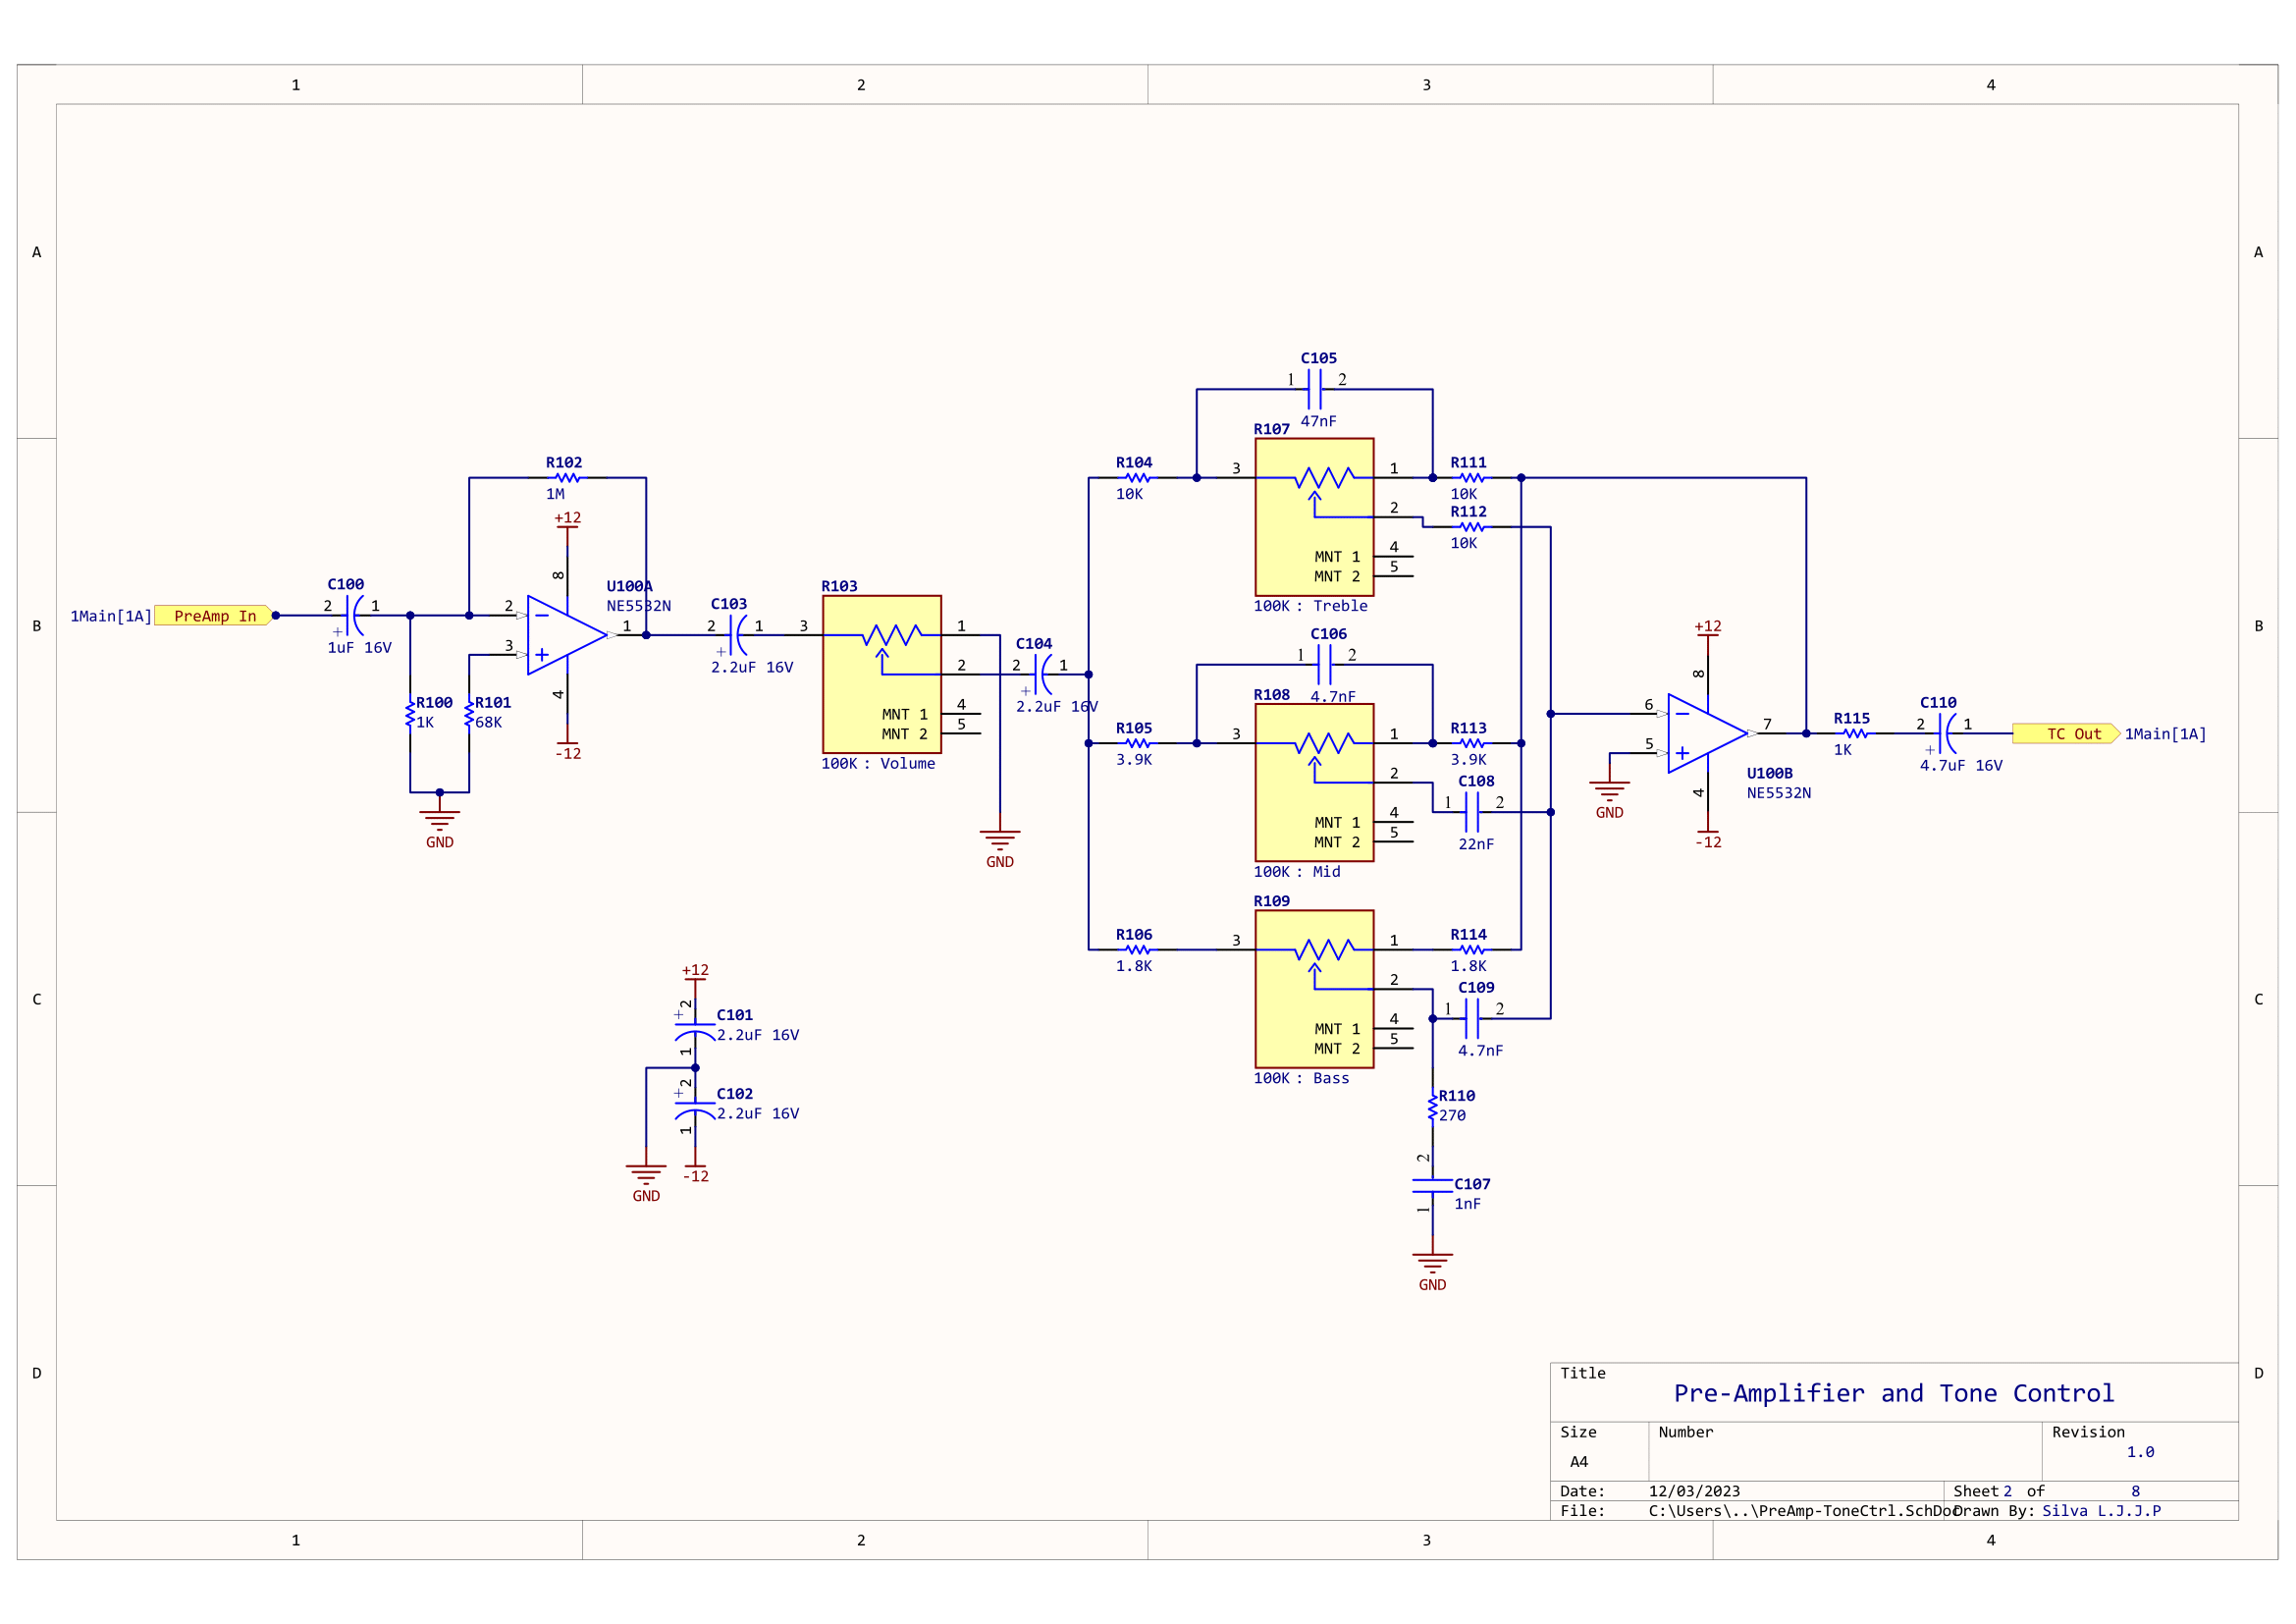
\includegraphics[scale=0.4]{preamp-sch.png}
                    \caption{Schematic of the Pre Amplifier and the Tone Controller}
                    \label{fig:enter-label}
                \end{figure}

            \subsection{Compressor}
                This effect can level the signal of the audio signal, so the audio signal does not have sudden dynamic variations, and the louder sounds and quieter sounds sound at closer levels. It requires the amplifier to have a large gain in smaller input signals and a smaller gain in large input signals.\\\\
                This is achieved by a basic non inverting amplifier, where the feedback resistors consists of a resistor and a light dependent resistor in parallel.\\\\
                The Output of the amplifier is rectified after amplifying, and then fed to drive an LED which is in contact with the LDR. The intensity of the LED increases with higher amplitudes, hence reducing the resistance in the LDR, an in combination the entire LDR, hence reducing the gain. For lower amplitudes as the resistance of LDR is very large the feedback resistance is closer to 220K$\Omega$.\\\\
                Here when rectifying the signal the LED is set in parallel with a capacitor, which smoothens out the rectified wave, hence reducing the sudden changes of the amplitude.\\\\
                Here germanium diodes are used in the diode bridge to further reduce the voltage drop.

                \begin{figure}
                    \centering
                    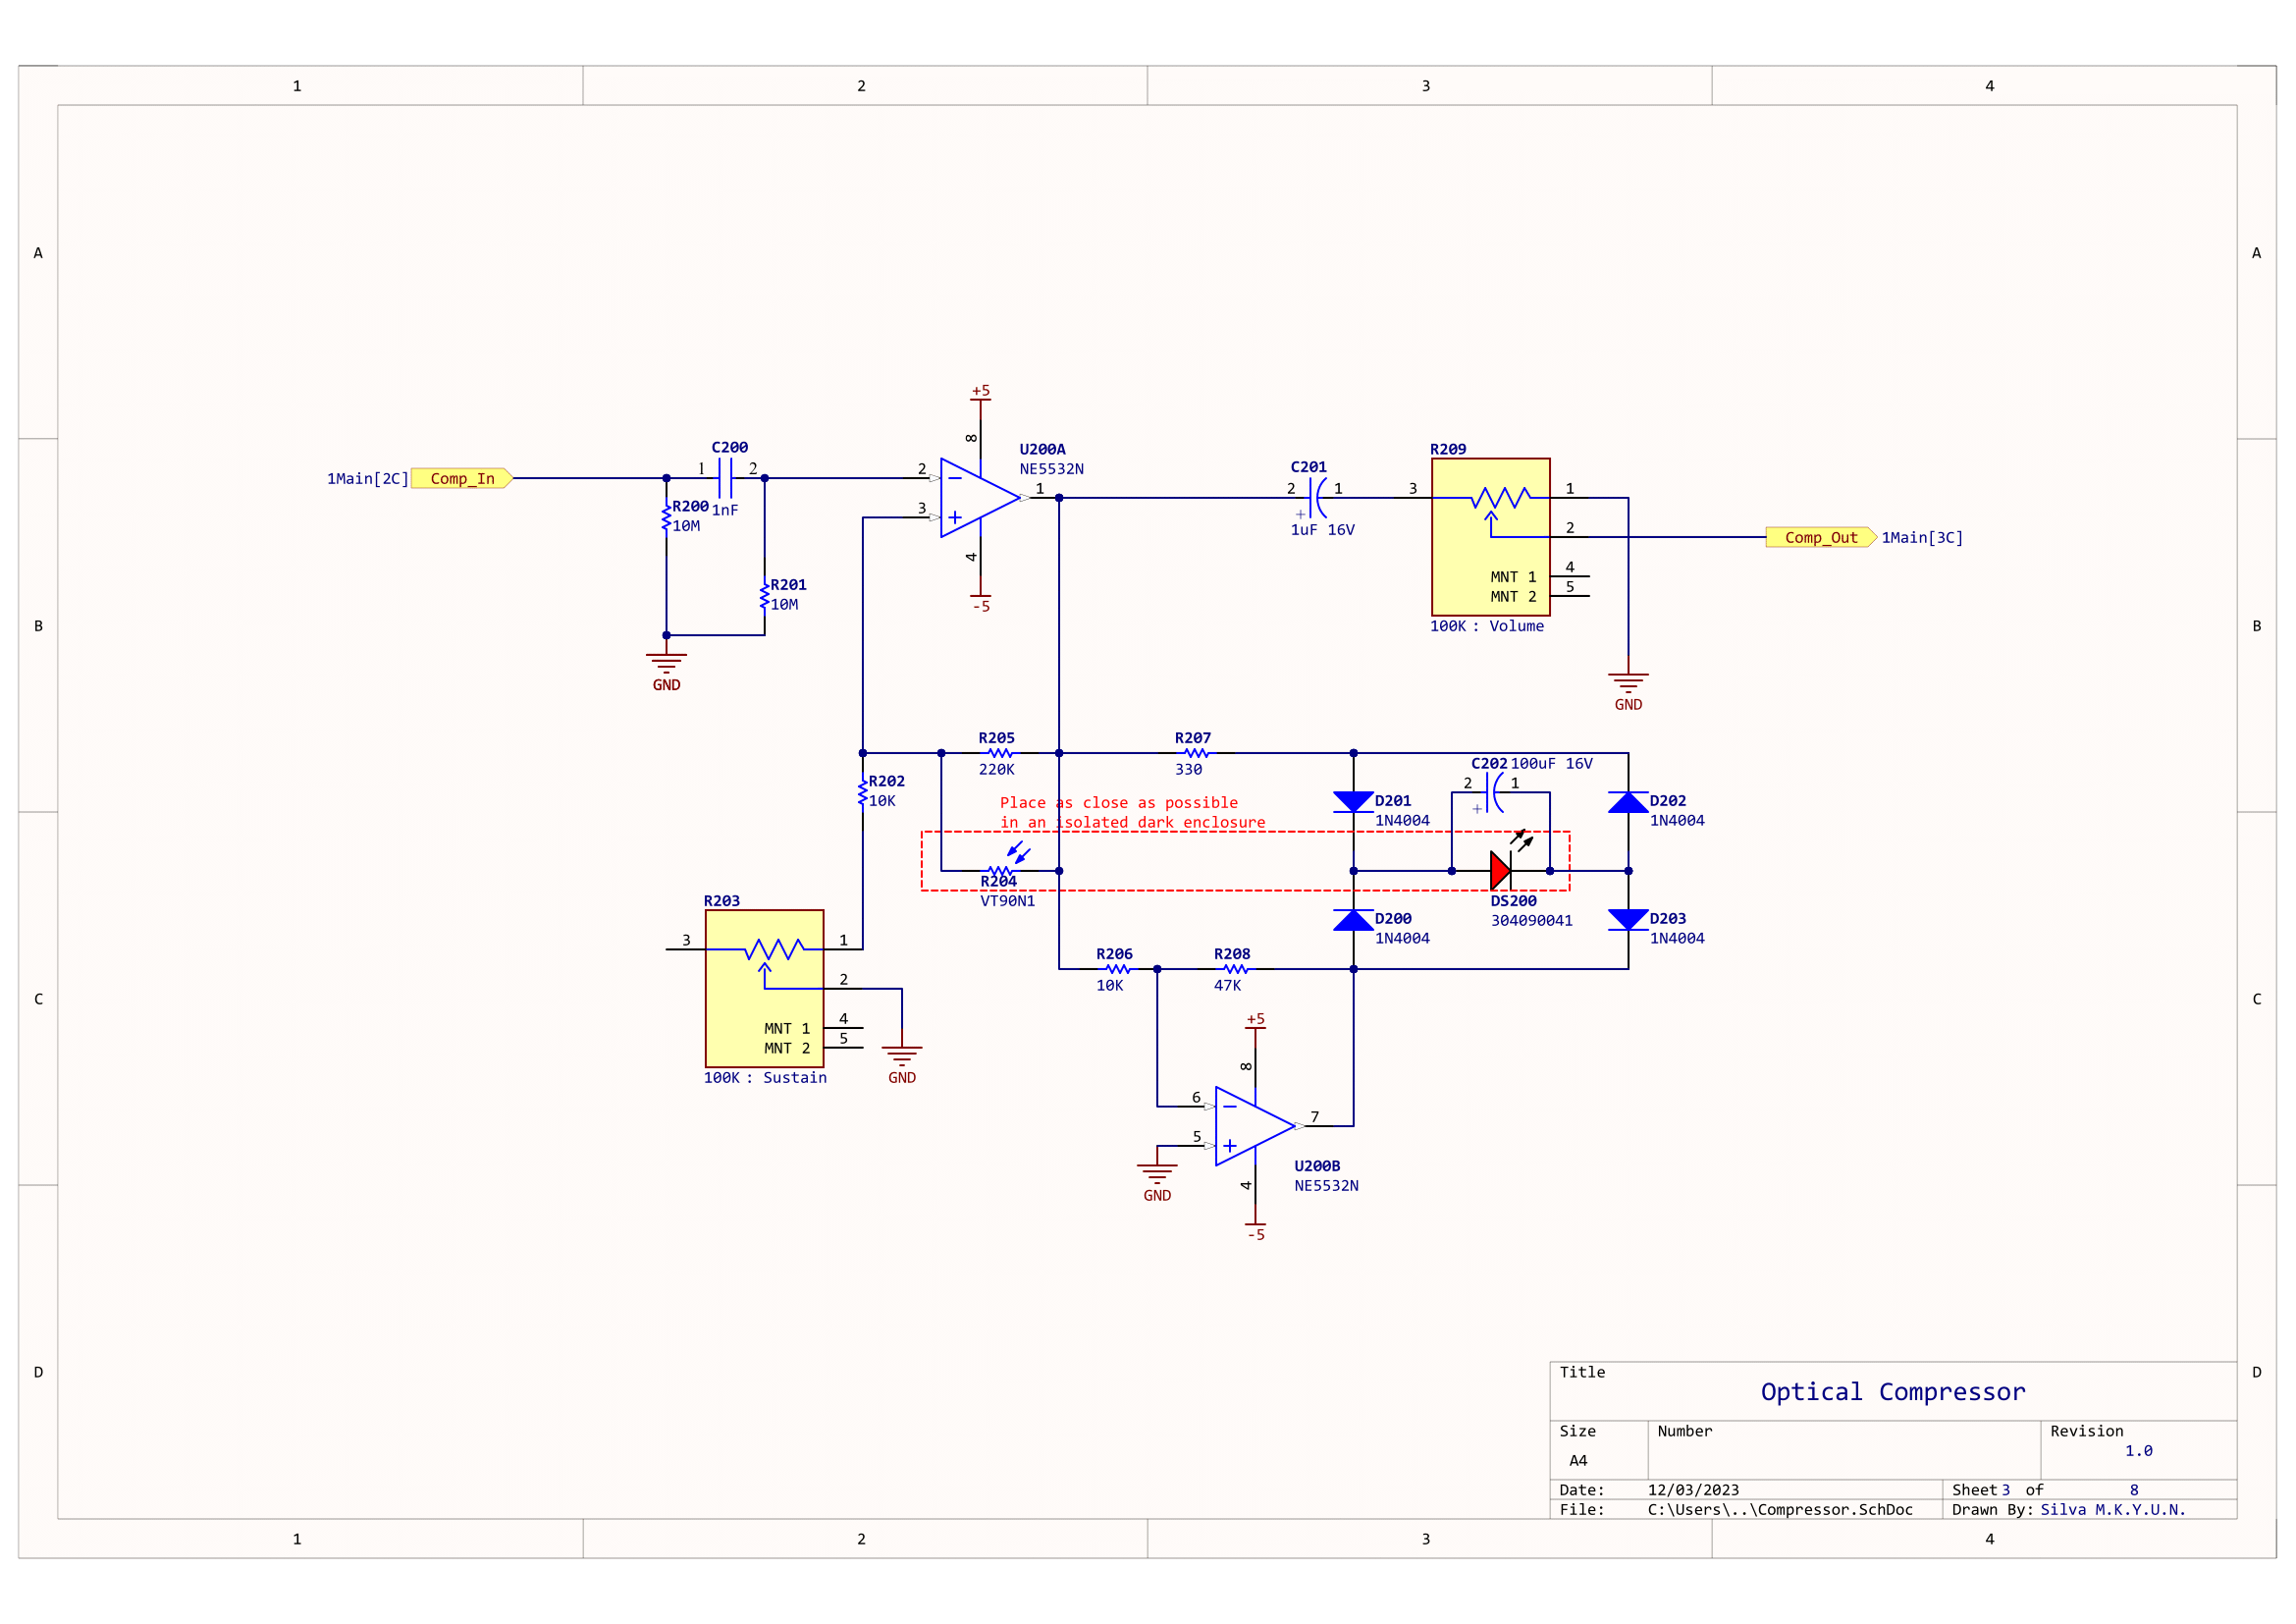
\includegraphics[scale=0.4]{compressor.png}
                    \caption{Schematic of the Compressor}
                    \label{fig:enter-label}
                \end{figure}

            \subsection{Wah}
                This effect can give the audio signal a resemblance to a human voicing a "wah-wah". This is done by sending the signal through a bandpass filter, and varying the center frequency back and forth when the player requires the effect.\\\\
                Here, the filter is a multiple feedback active filter created using an operational amplifier. The center frequency can be changed by changing the value of the resistor that connects between the \textit{\texttt{Wah\_pedal\_in}} net of the following schematic, and the ground. The circuit used here is a simplified circuit equivalent to very complex Wah pedals, which often use inductors and capacitors to create filters.\\\\
                
                \begin{figure}[h!]
                    \centering
                    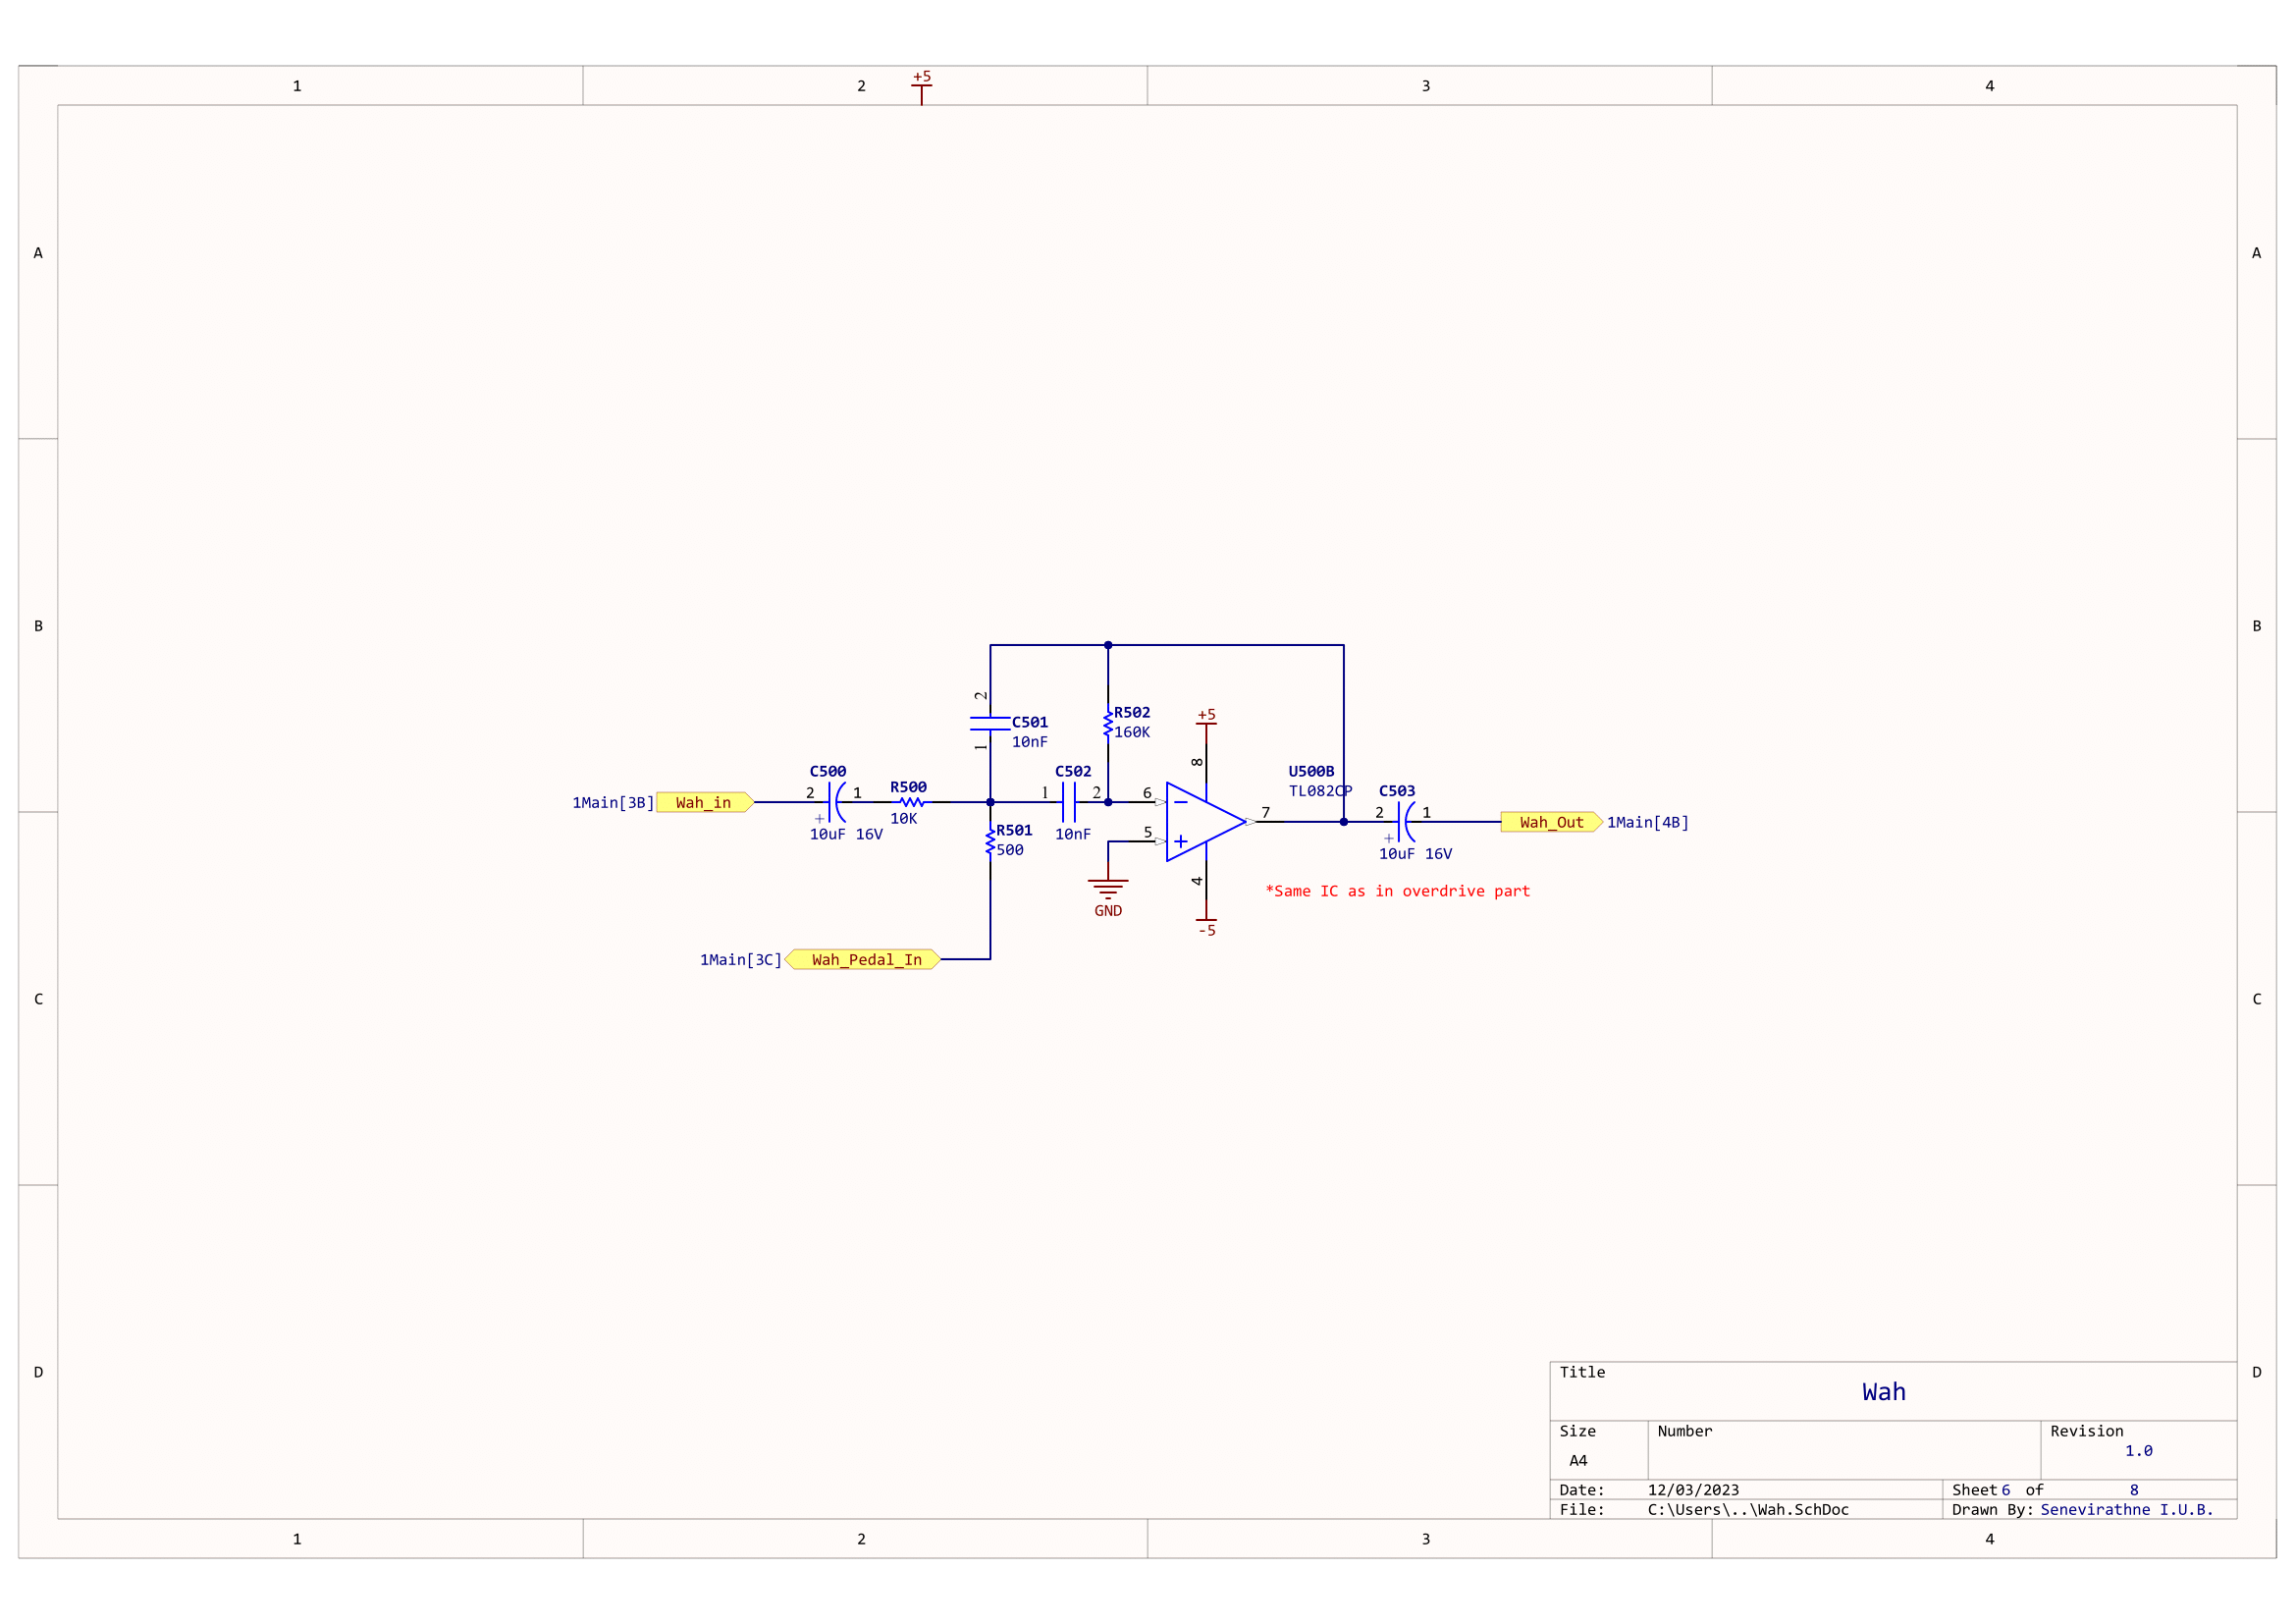
\includegraphics[scale=0.4]{Wah.png}
                    \caption{Schematic of the Wah}
                    \label{fig:enter-label}
                \end{figure}
                
                As this effect requires the user to change the resistance of potentiometer while playing the instrument, a foot-pedal is provided. This is the method used by a vast number of manufacturers.

            \subsection{Overdrive/Distortion}
                This is an effect which can give the audio a gritty and a distorted sound. This is achieved by saturating the signal using diodes.\\
                There are two types of distortions known as Soft Clipped and Hard Clipped. Soft Clipped Distortion reduces the peaks of the signal gradually, while the Hard Clipped Distortion clips the wave directly with no smoothing.\\
                Here this is achieved by filtering out the low frequency content in the signal using an active low pass filter constructed using an operational amplifier, and the clipping the feedback of the above filter. Distortion is achieved by simply clipping the total output wave from the above low pass filter. Both of these clippings are done by using a pair of diodes in opposite direction.

                \begin{figure}[h!]
                    \centering
                    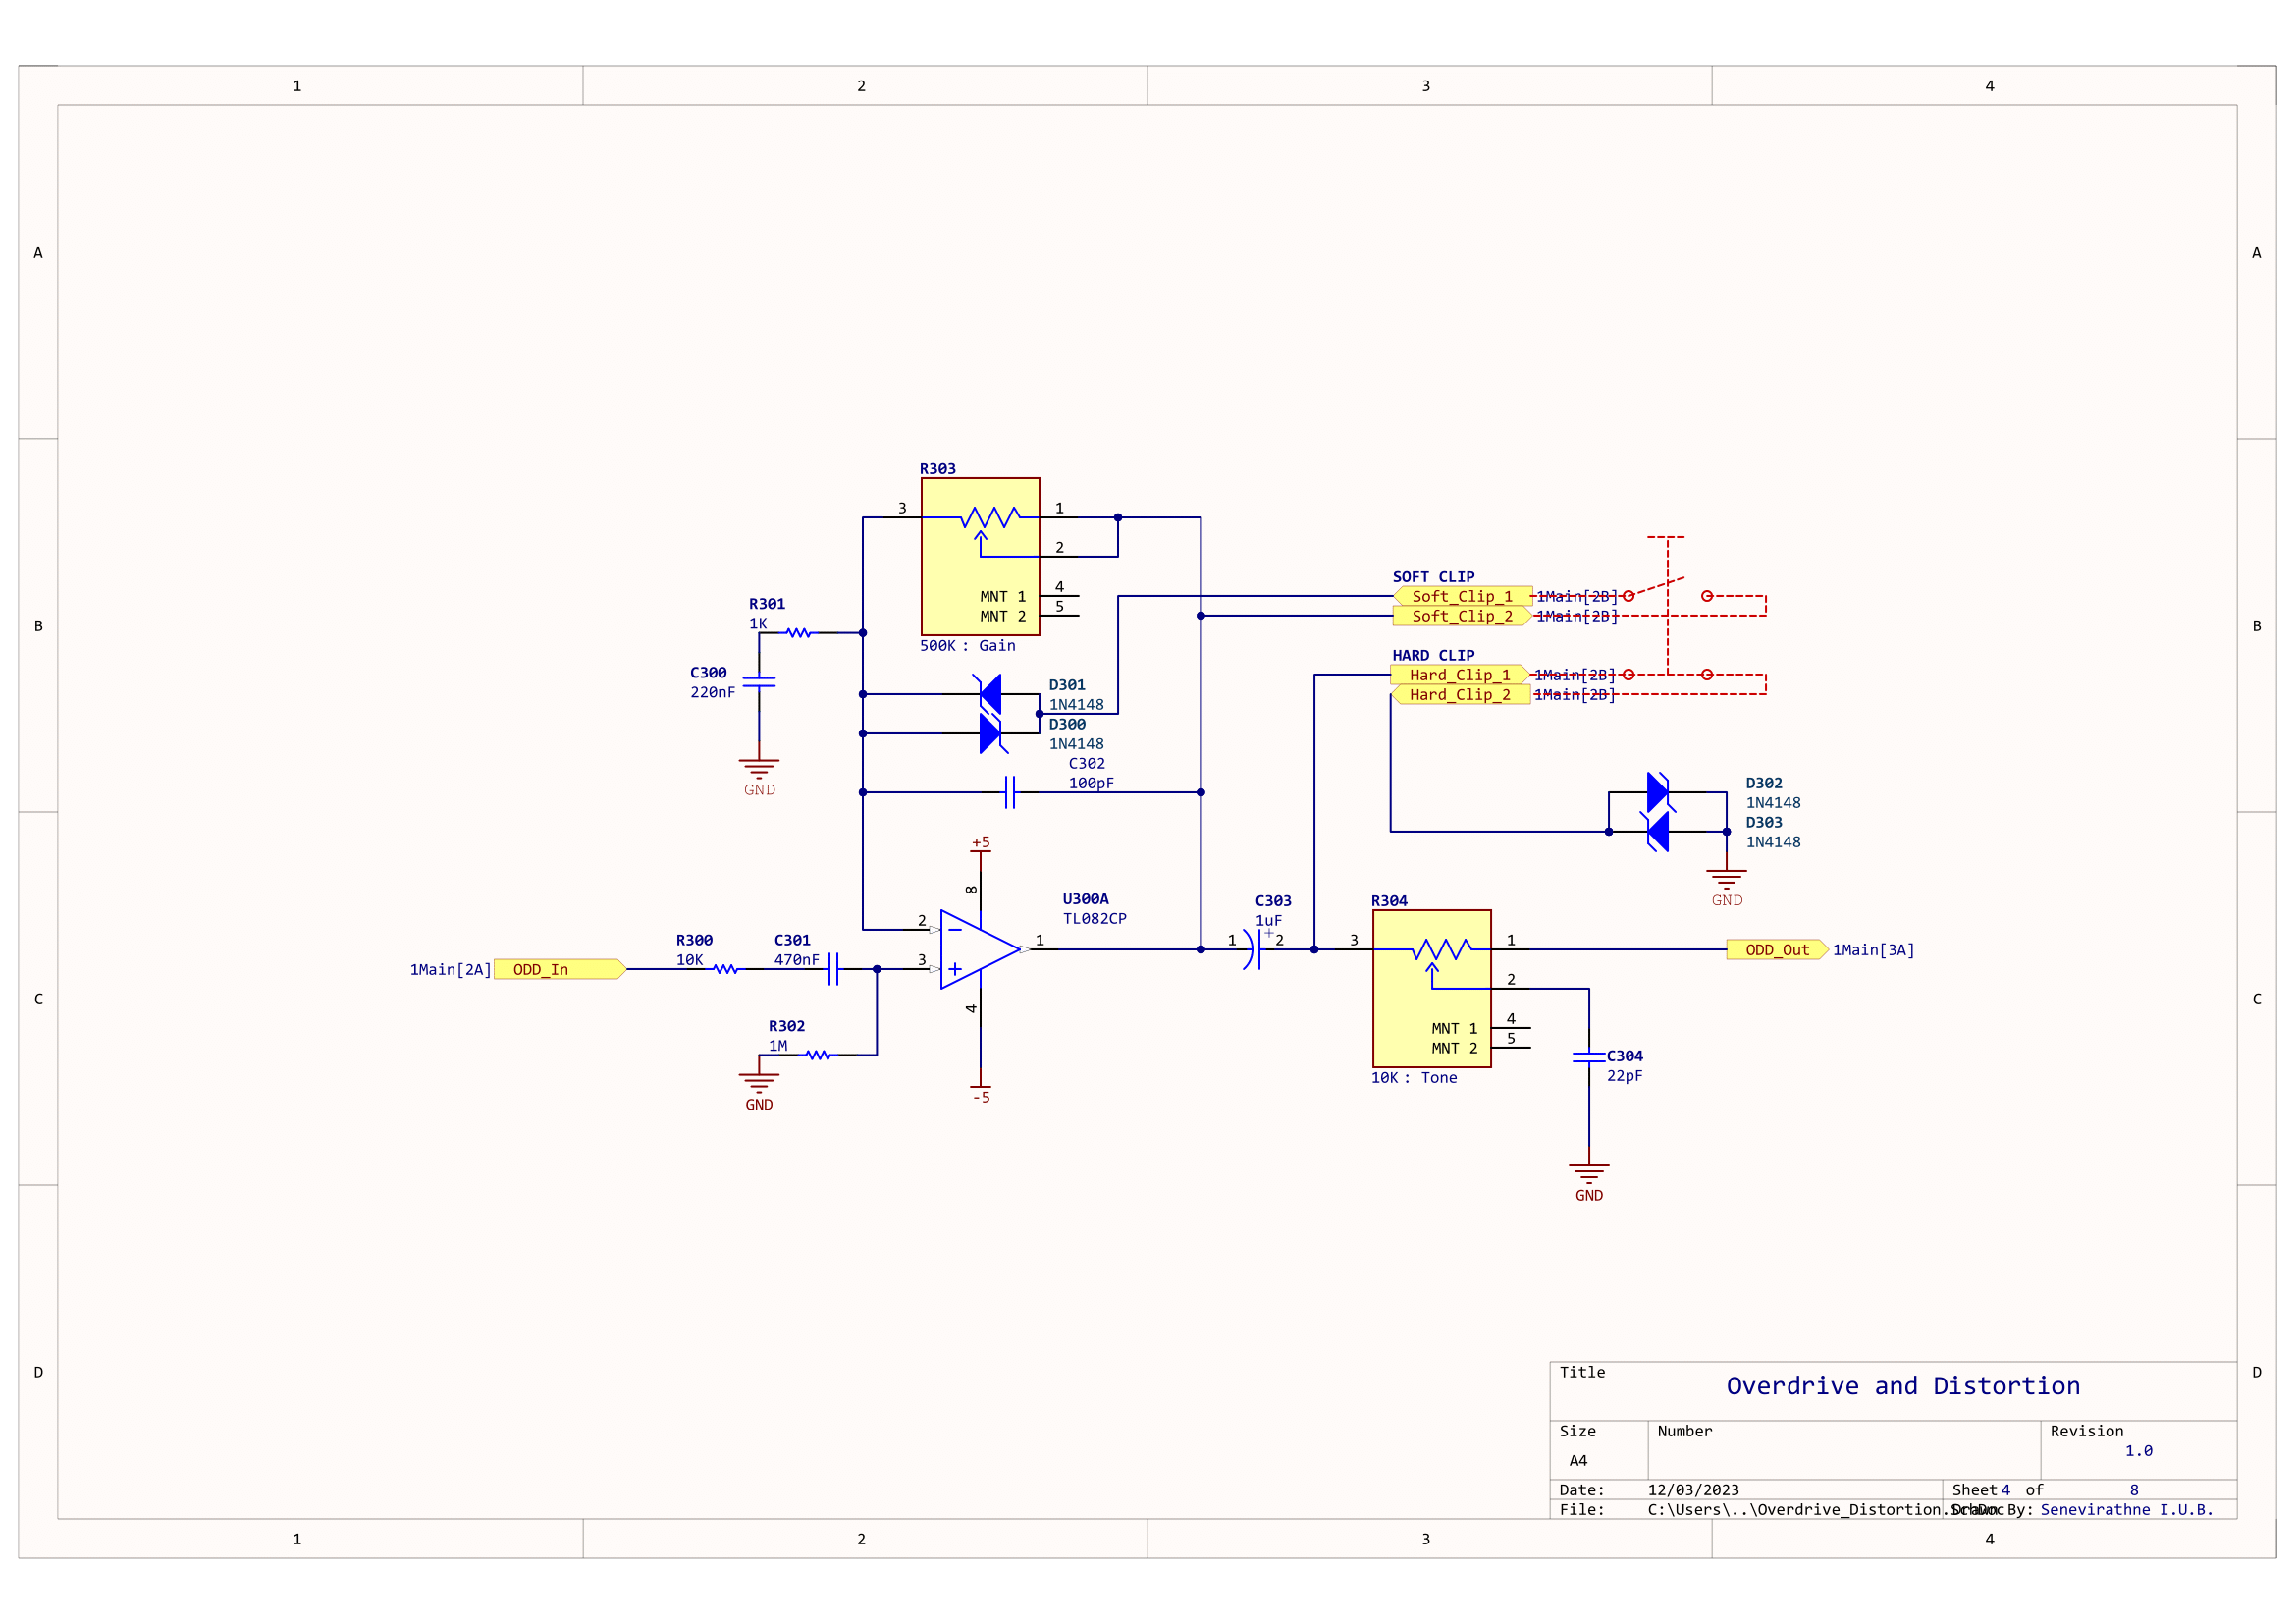
\includegraphics[scale=0.4]{odd.png}
                    \caption{Schematic of the Overdrive and Distortion}
                    \label{fig:enter-label}
                \end{figure}

            \subsection{Fuzz}
                Fuzz pedal can give the a 'fuzzy and warm' tone to the audio, and an attempt for the replication of old damaged amplifiers containing damaged electrical components or broken speakers.\\
                
                \begin{figure}
                    \centering
                    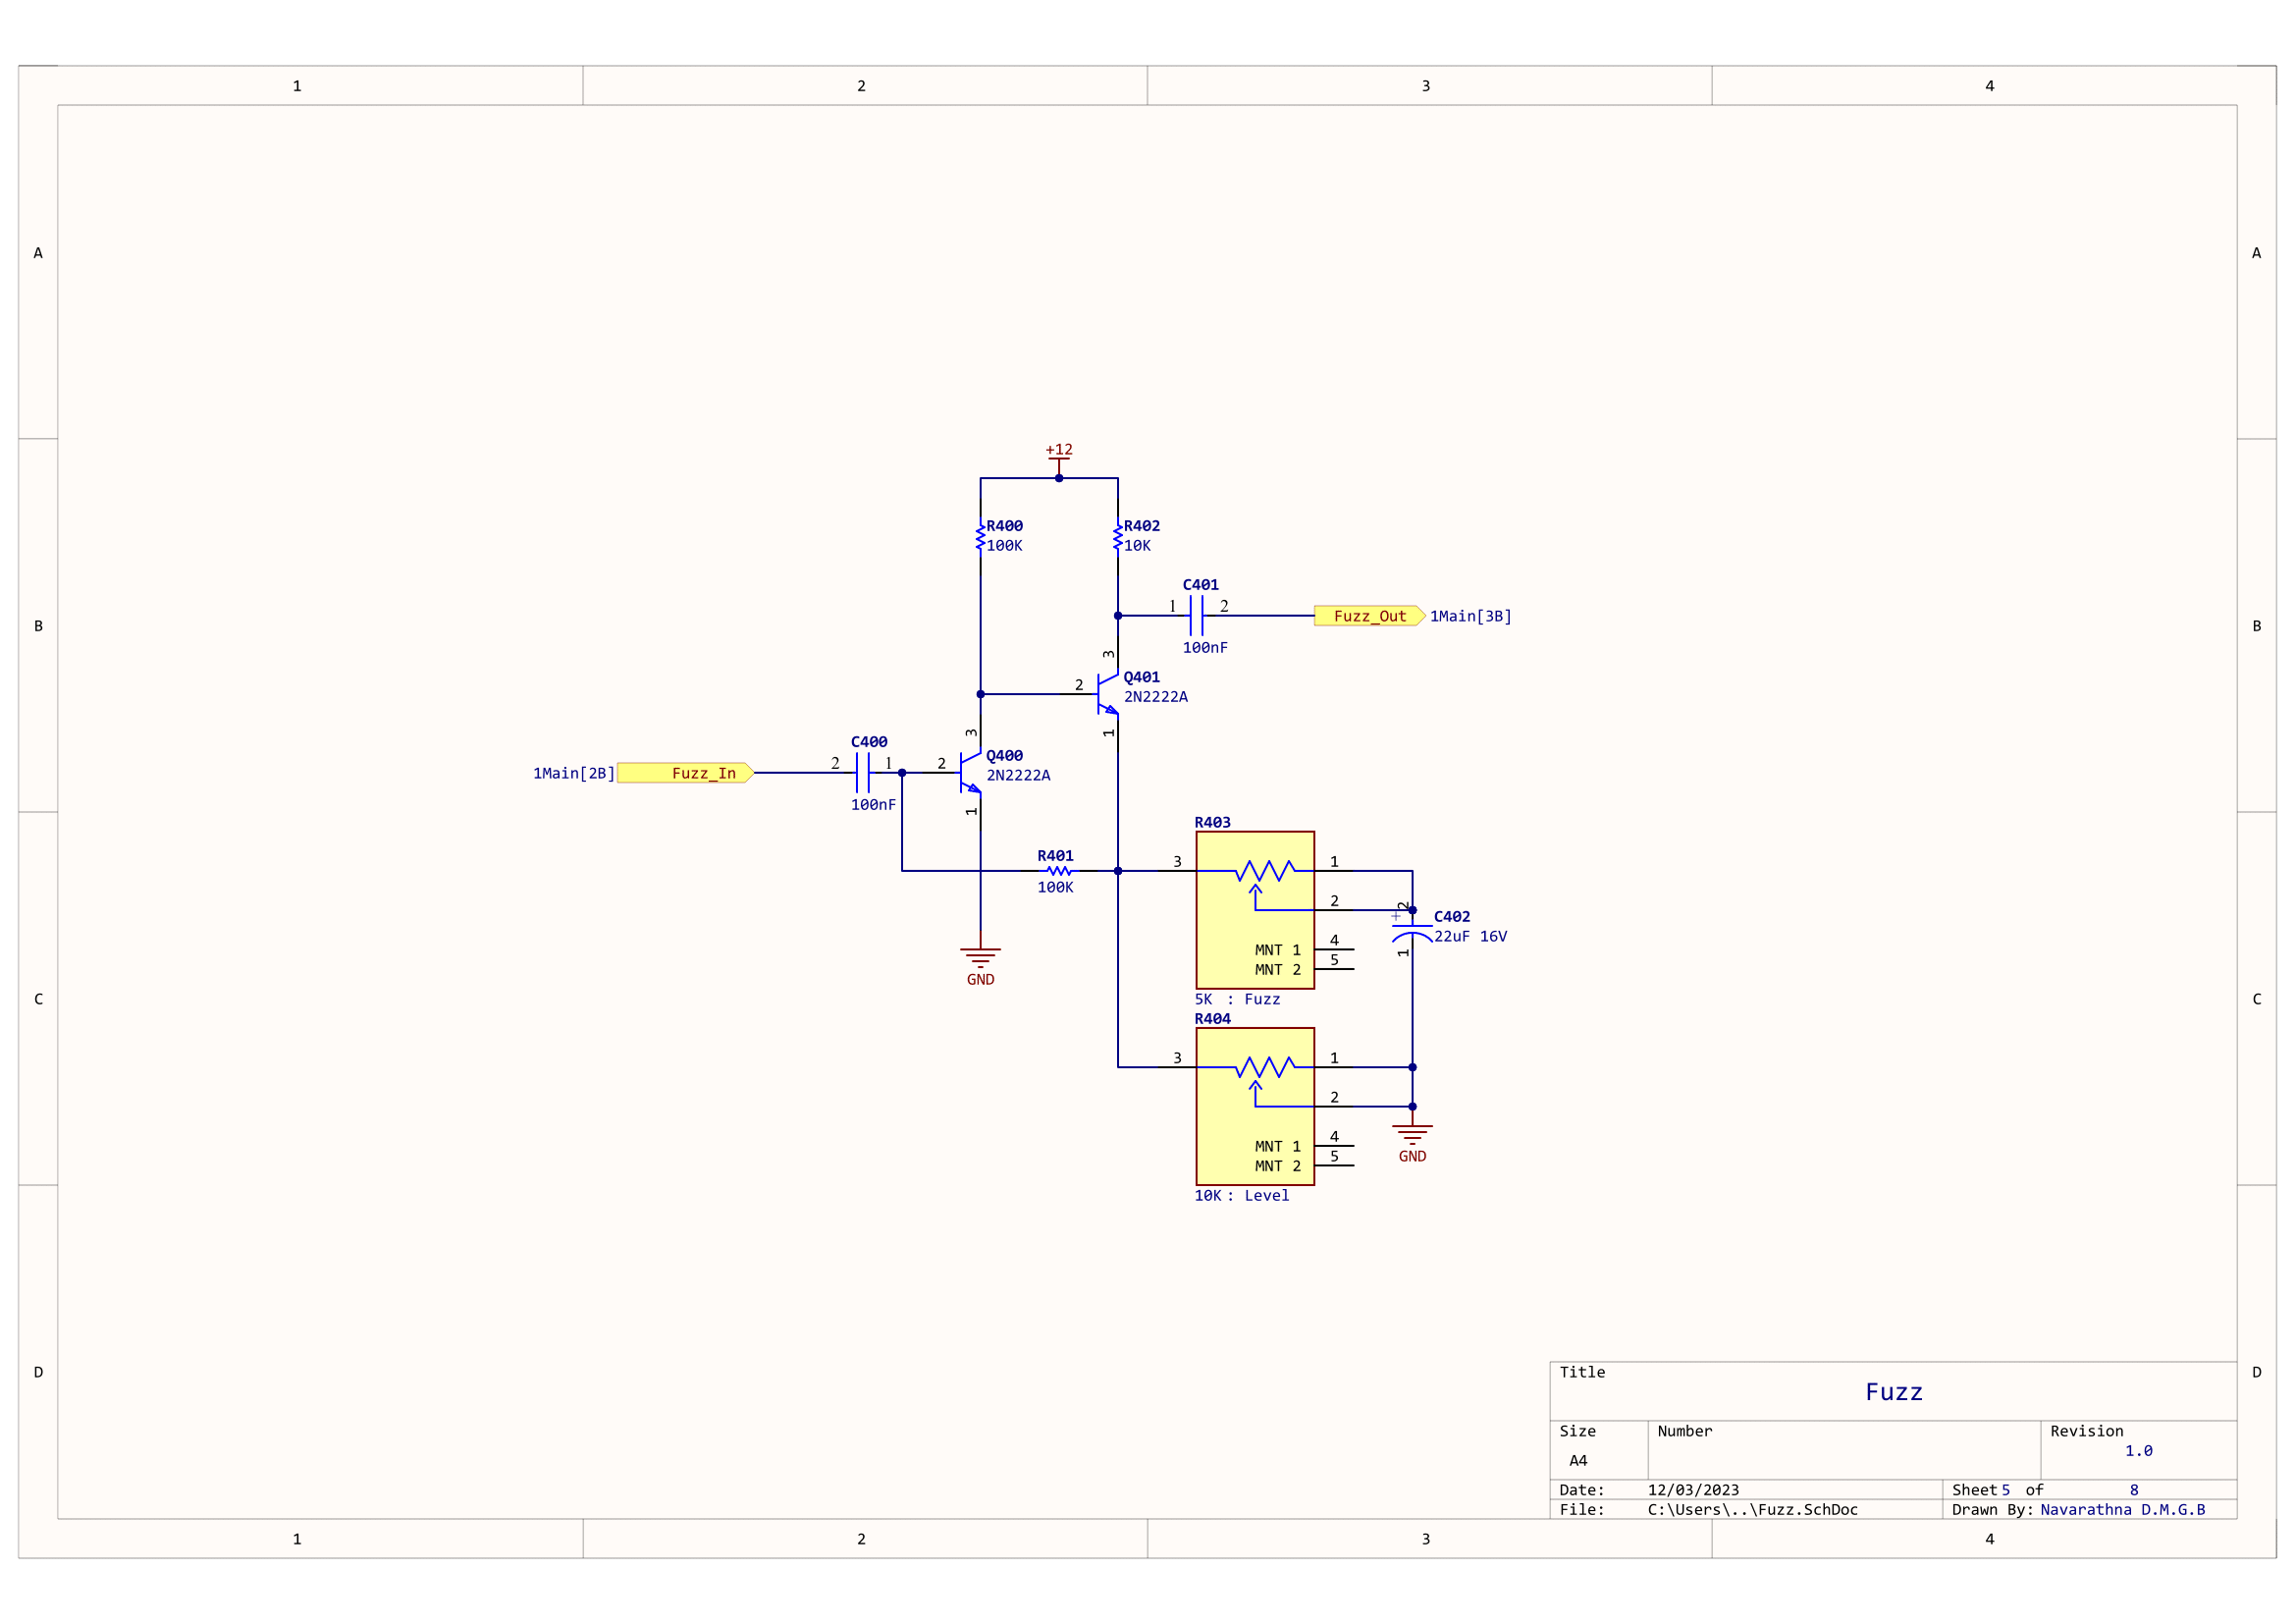
\includegraphics[scale=0.4]{fuzz.png}
                    \caption{Schematic of the Fuzz}
                    \label{fig:enter-label}
                \end{figure}
                
                This is achieved by sending the signal through two bi-junction transistors in Common Emitter mode with feedback to the first transistor. These transistors are set in such a way that higher amplitude signals the transistor briefly enters the saturation mode, giving the 'fuzzy' sound.
                
            \subsection{Tremolo}
                Tremolo effect resemble the player turning the volume high to low to high, repeatedly. This is done by modulating the audio signal amplitude with an sine, square or a triangle wave.\\

                In the circuit we have used, first part is a triangle wave generator. This has been achieved by a low frequency oscillator created with an operational amplifier. The op amp has been used in comparator mode. When in the high output, the capacitor is getting charged through the feedback resistor, and when the voltage becomes higher than the non inverting terminal, the output gets low as the capacitor is connected to the inverting terminal, and the capacitor gets discharged. Above charging and discharging cycle leads to a triangular wave. \\

                After this, the output is sent through an LC filter to smoothen this into a sine wave. Then this is biased using the divider bias method, and fed into the base of a transistor, where the emitter is connected to the ground, and the collector is connected to an amplified output: hence shorting the signal to the ground, modulating the amplitude of the signal.
  
                \begin{figure}
                    \centering
                    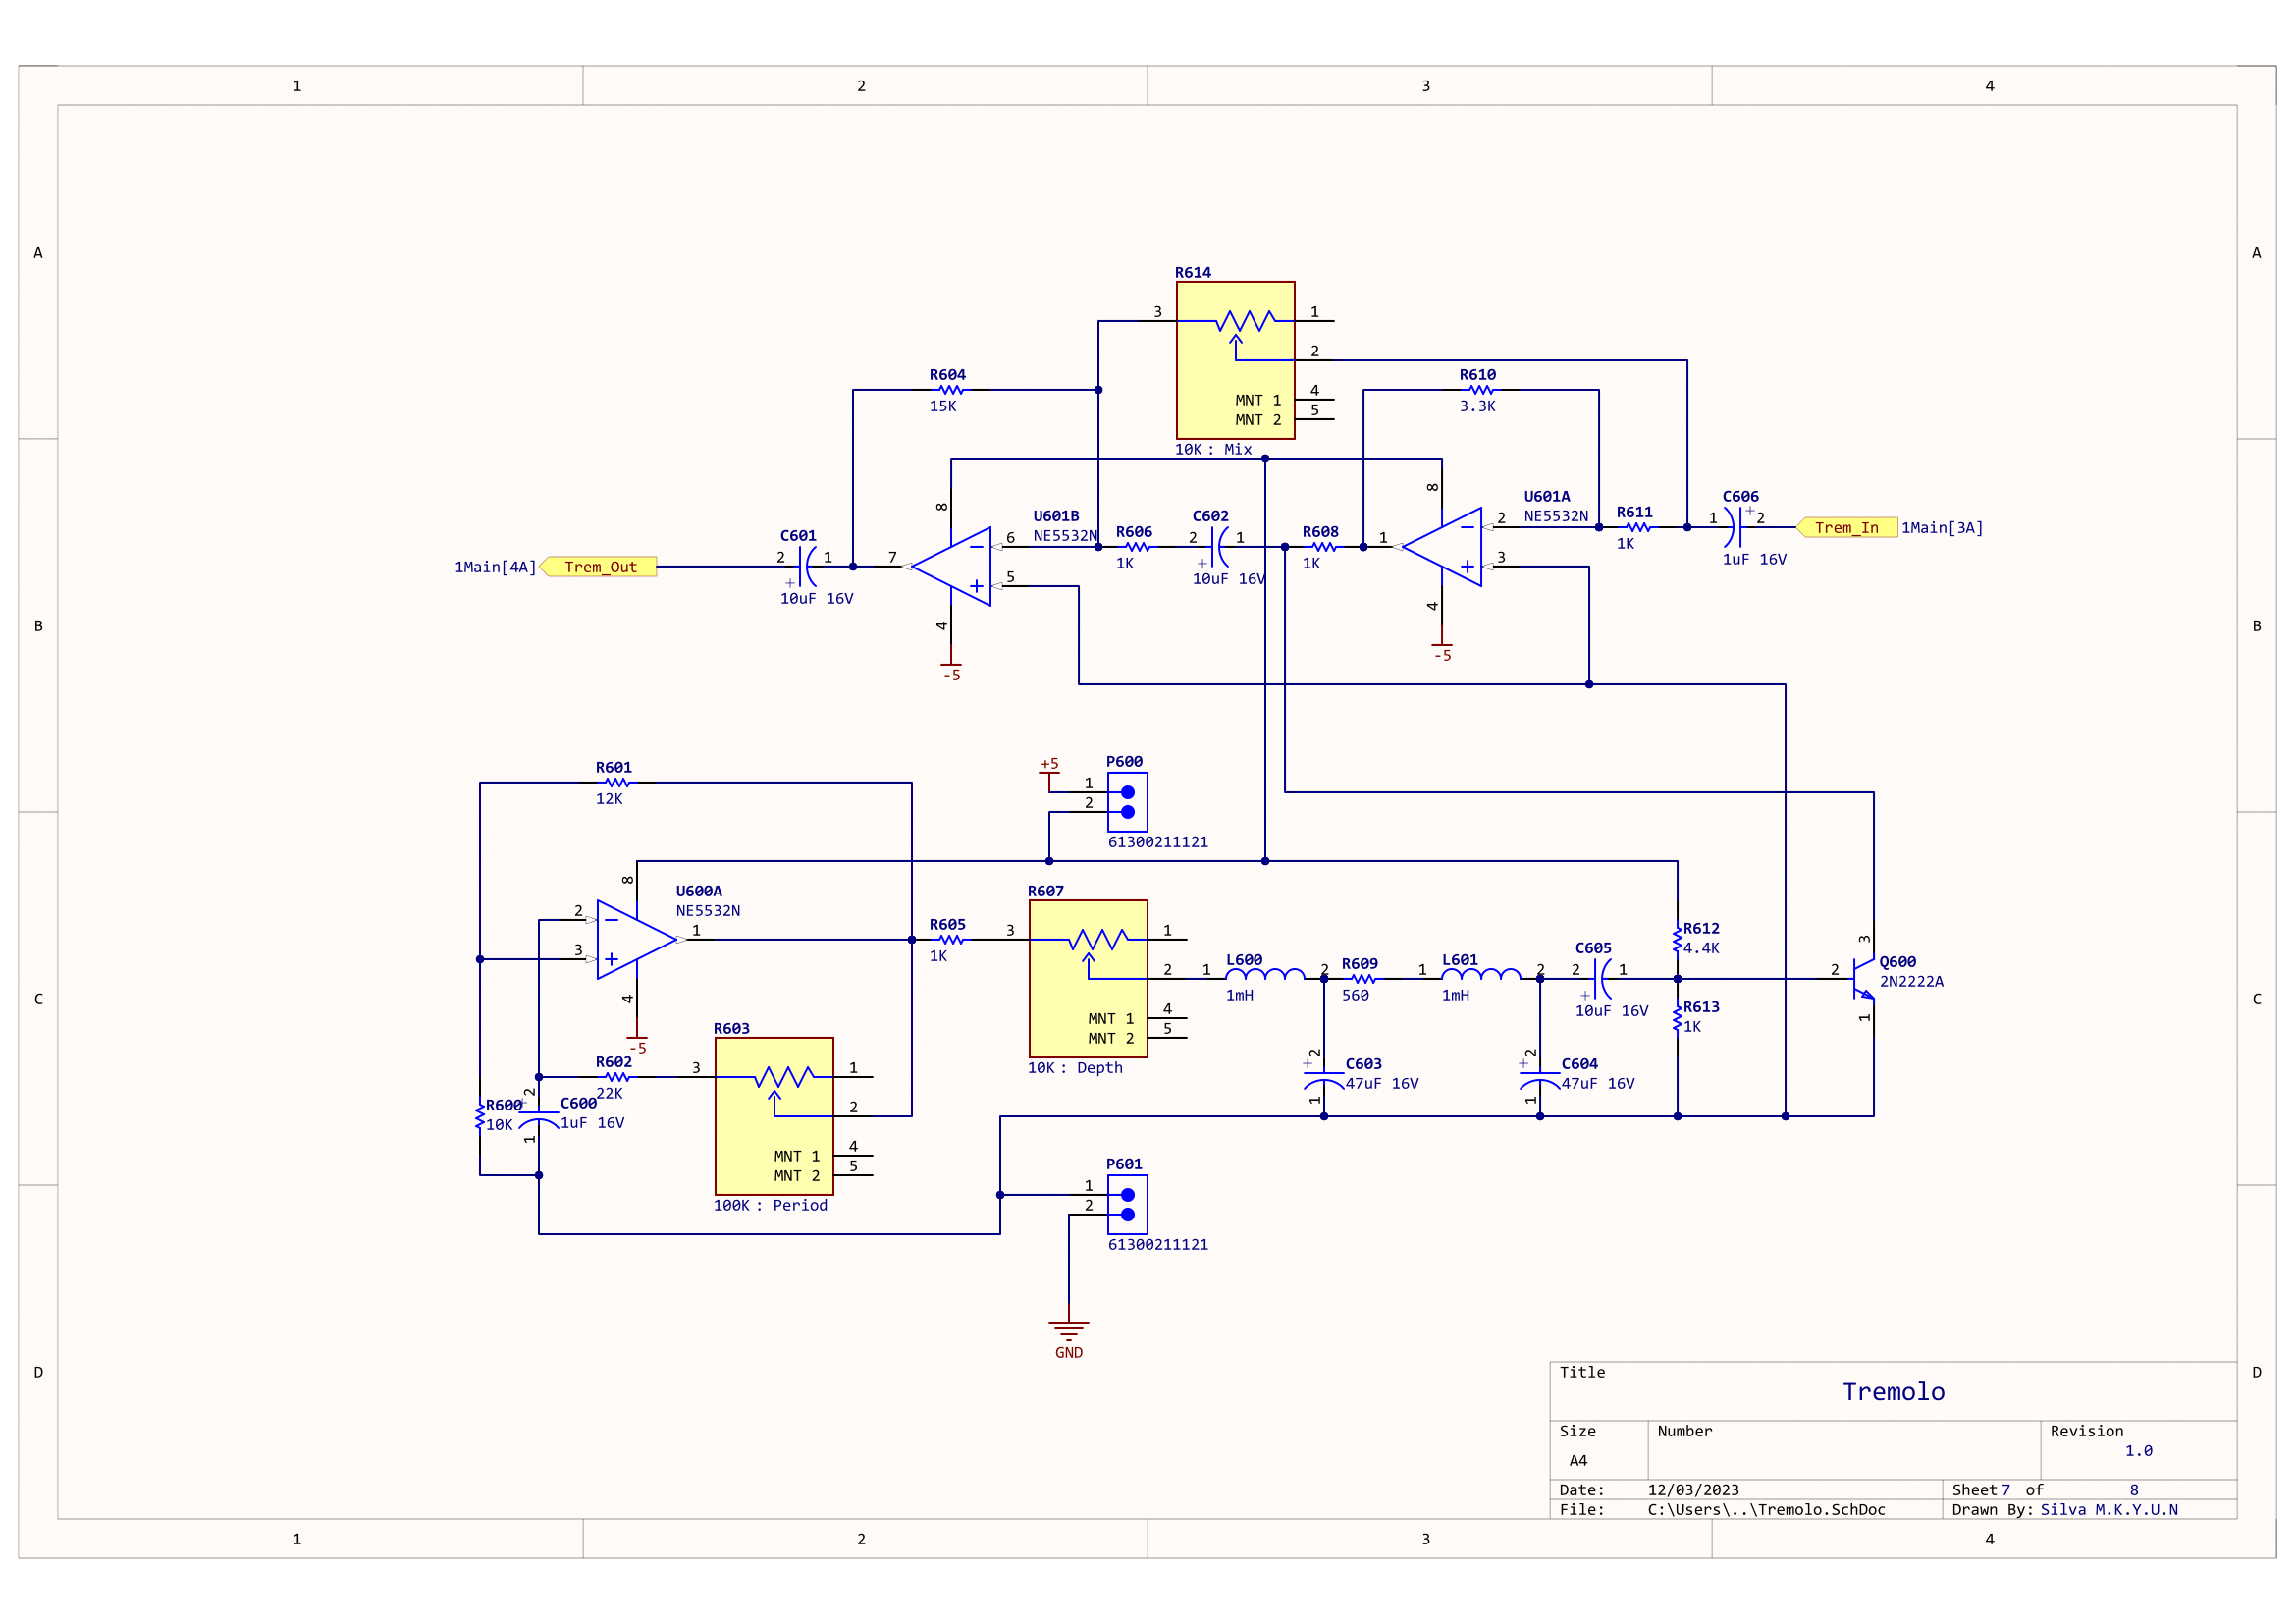
\includegraphics[scale=0.4]{tremolo.png}
                    \caption{Schematic of the Tremolo}
                    \label{fig:enter-label}
                \end{figure}
                
            \subsection{Power Amplifier}
                Power amplifier consists of 2 stages. First stage provides all necessary voltage gain to get desirable voltage to drive the output stage(push-pull amplifier). In the first stage we have used an operational amplifier (TDA2040) with closed loop voltage gain of 9.33.\\

                Two additional diodes are used to prevent any damages to the load(speaker) if it was to experience a unstable high voltage. diodes let through current only for a certain voltage point and by doing so they keep the voltage stable at that point.
                \begin{figure}
                    \centering
                    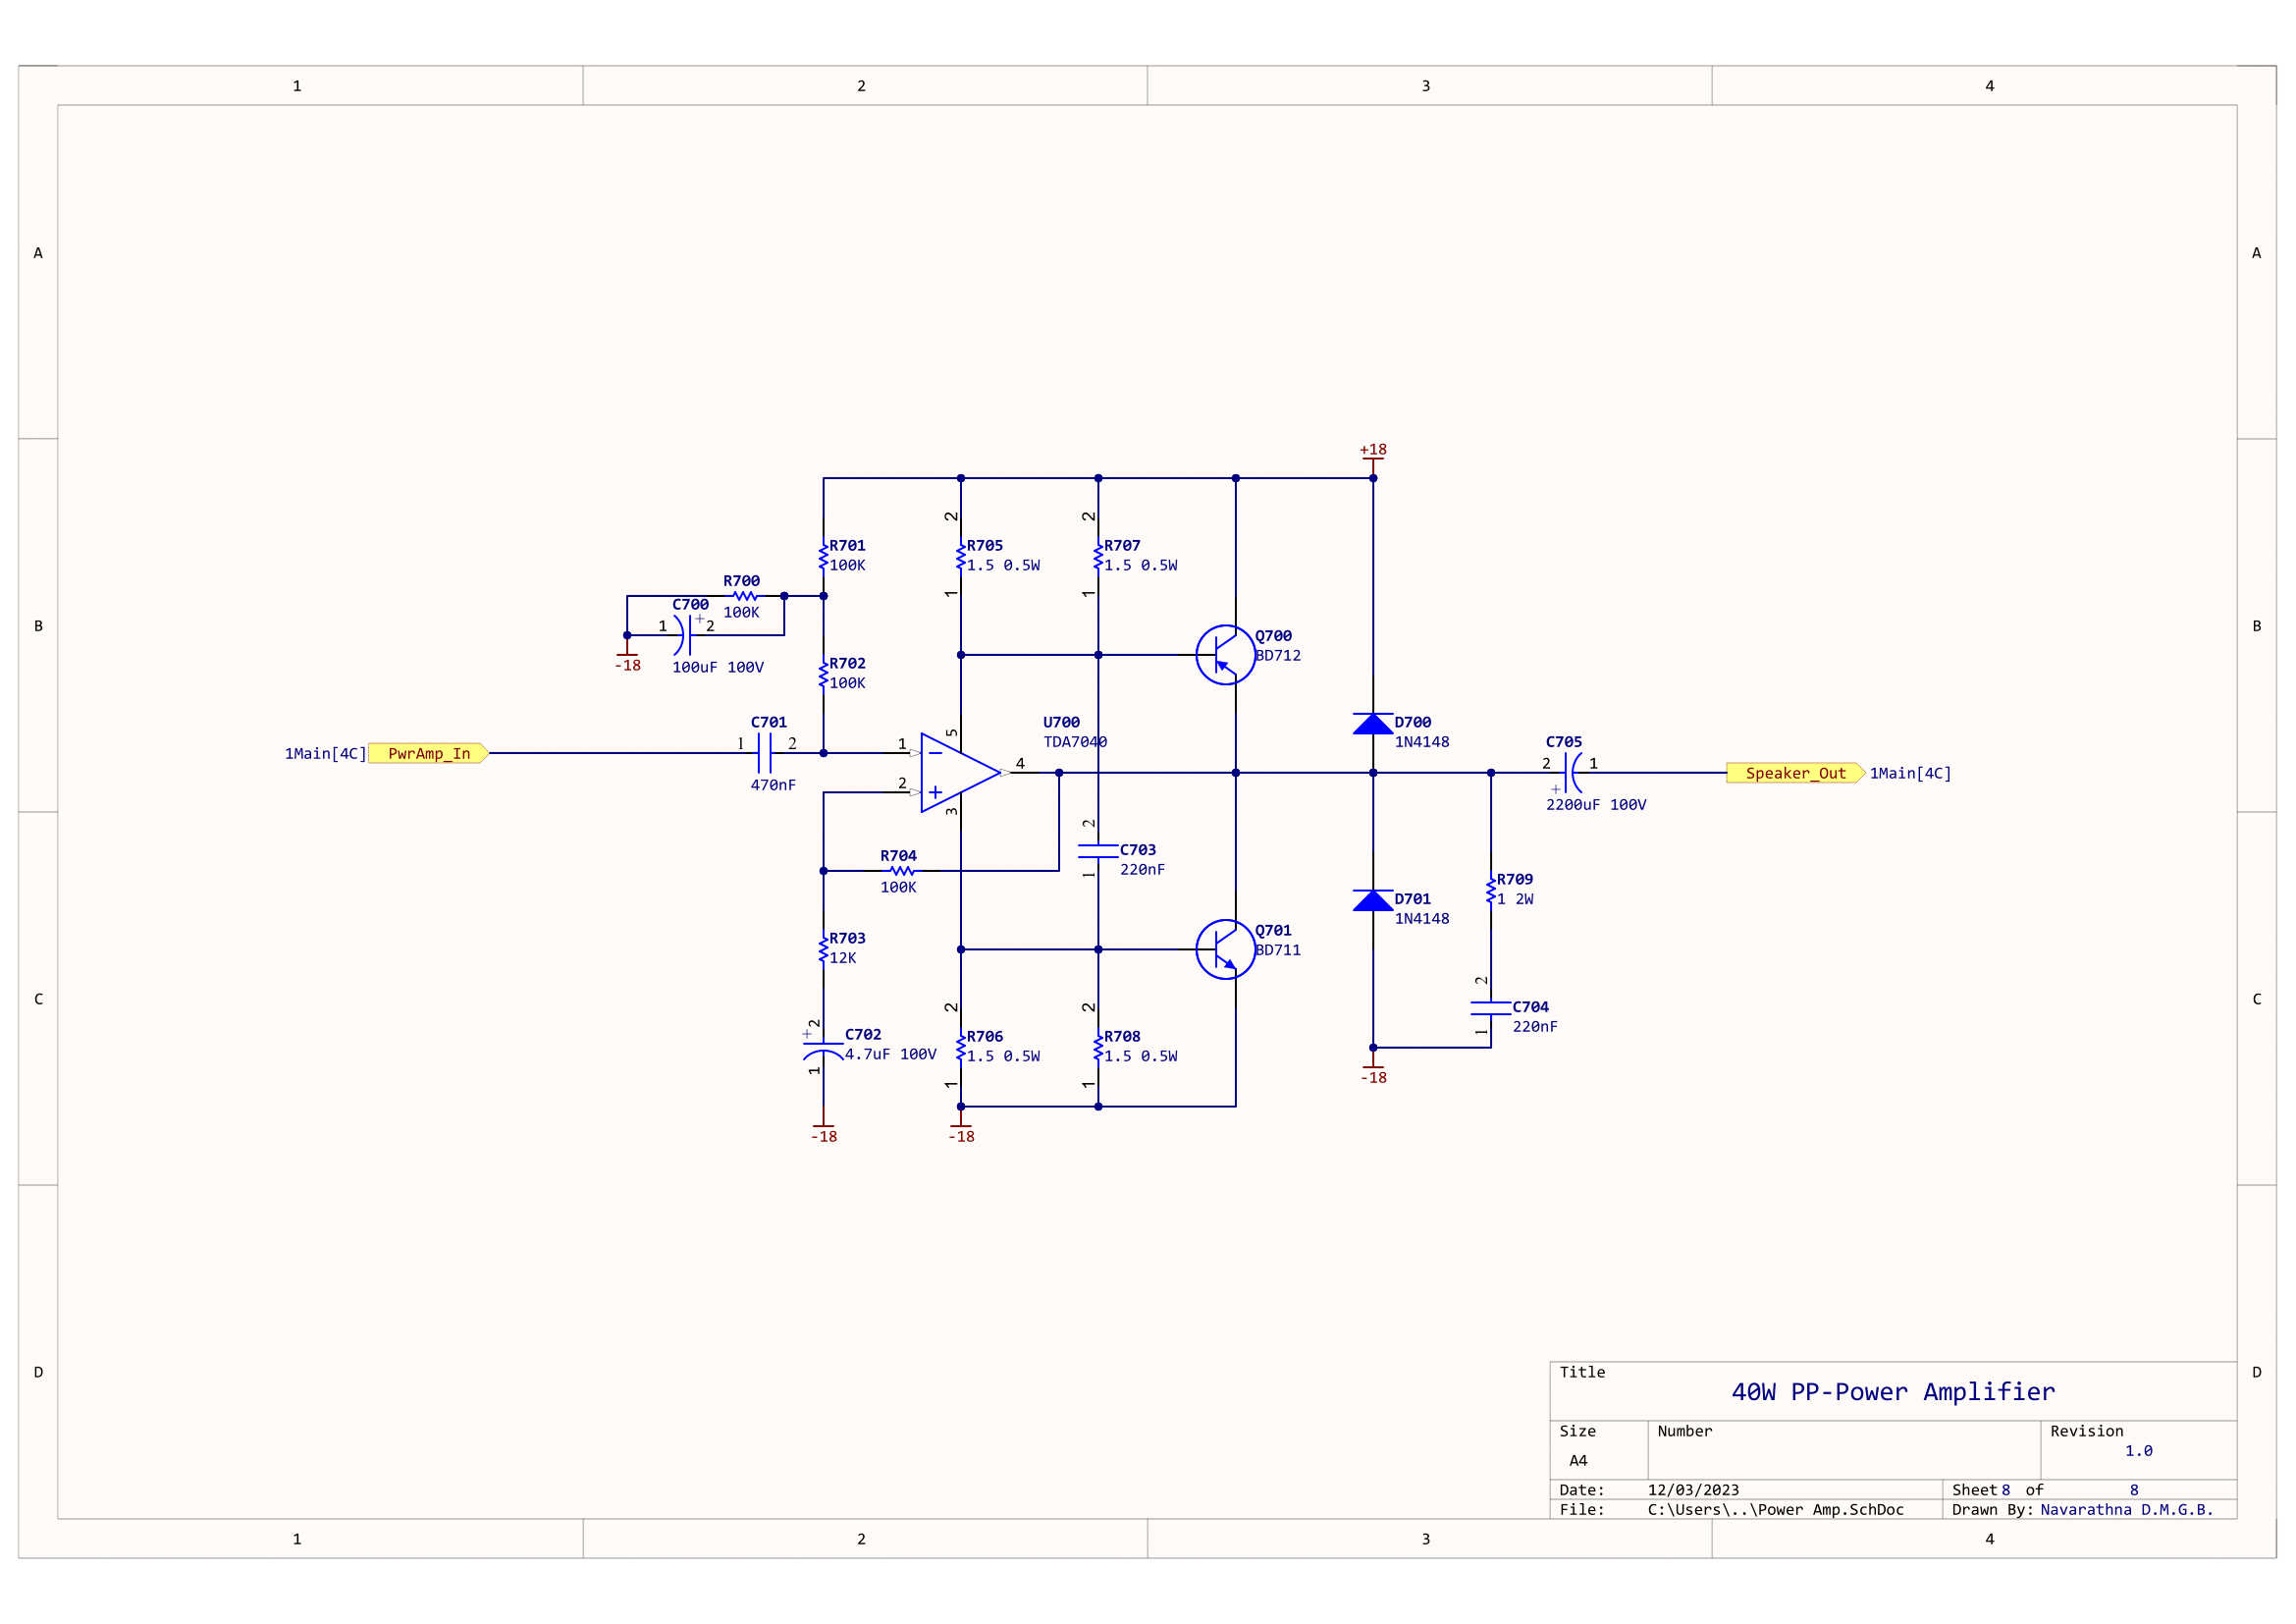
\includegraphics[scale=0.4]{poweramp.png}
                    \caption{Schematic of the Power Amplifier}
                    \label{fig:enter-label}
                \end{figure}
                
            \subsection{Power Supply}
            Above circuits require voltages +18V, -18V, +12V, -12V, +5V, -5V. This has been obtained by a dual power supply cascading from 18V to 12v to 5V. The input to this circuit is from a 230V to 24Vx2 0.5A centre tapped step down transformer.\\
            The power is regulated using the regulators LM7805, LM7812, LM7818, LM7905, LM7912 and LM 7918. These regulators, followed with large capacitors ensure that the ripple is minimal, so that the 50Hz ripple does not get mixed in with the audio signal.
                \begin{figure}[h!]
                    \centering
                    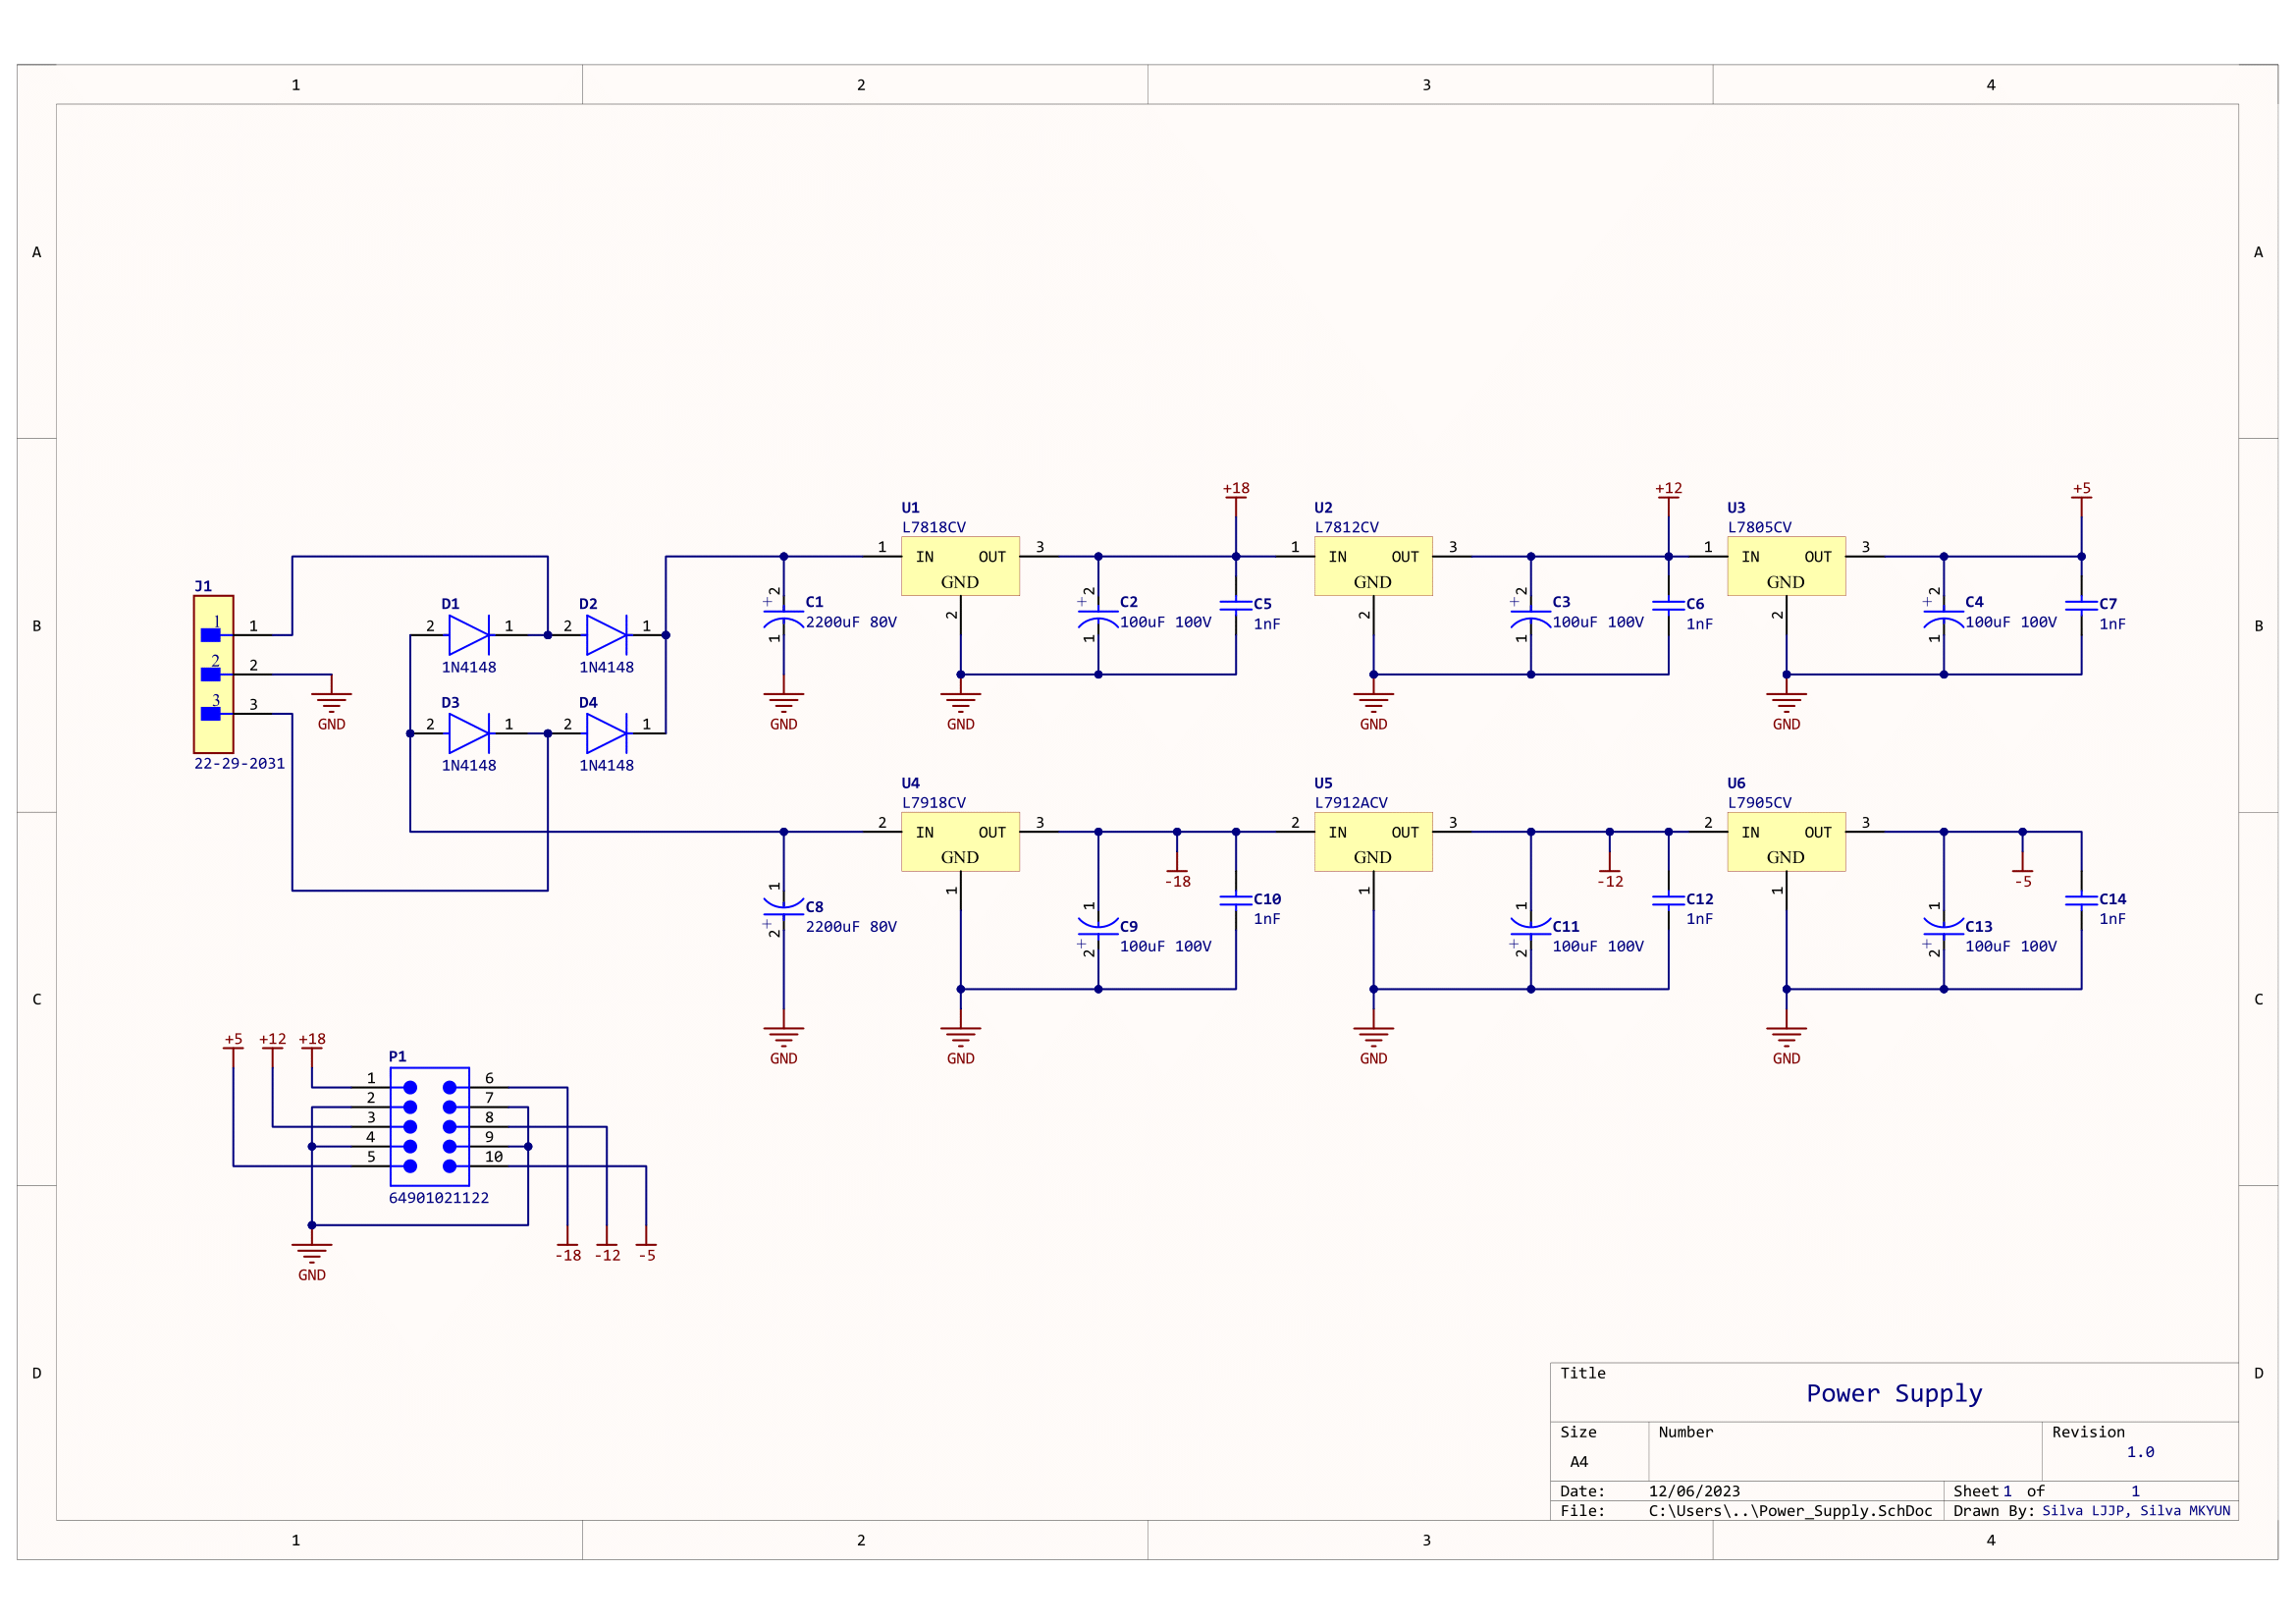
\includegraphics[scale=0.4]{ps-1.png}
                    \caption{Schematic of the Power Supply}
                    \label{fig:enter-label}
                \end{figure}
                
            \subsection{Interconnections between circuits}
                Above circuits are lined up in the following order:
                \begin{enumerate}
                    \item Pre Amplifier
                    \item Tone Controller
                    \item Compressor
                    \item Wah
                    \item Overdrive/Distortion
                    \item Fuzz
                    \item Tremolo
                    \item Power Amplifier
                \end{enumerate}

                In the earlier plans, it was decided to allow the user to switch between the effects by adding 6 rotary switches above each effect. But as this would complicate the circuit, require longer tracks, and require under-the component soldering (given this is done in single layer), it was decided to opt out this option. A simpler method would require digital electronics.\\

                \begin{figure}
                    \centering
                    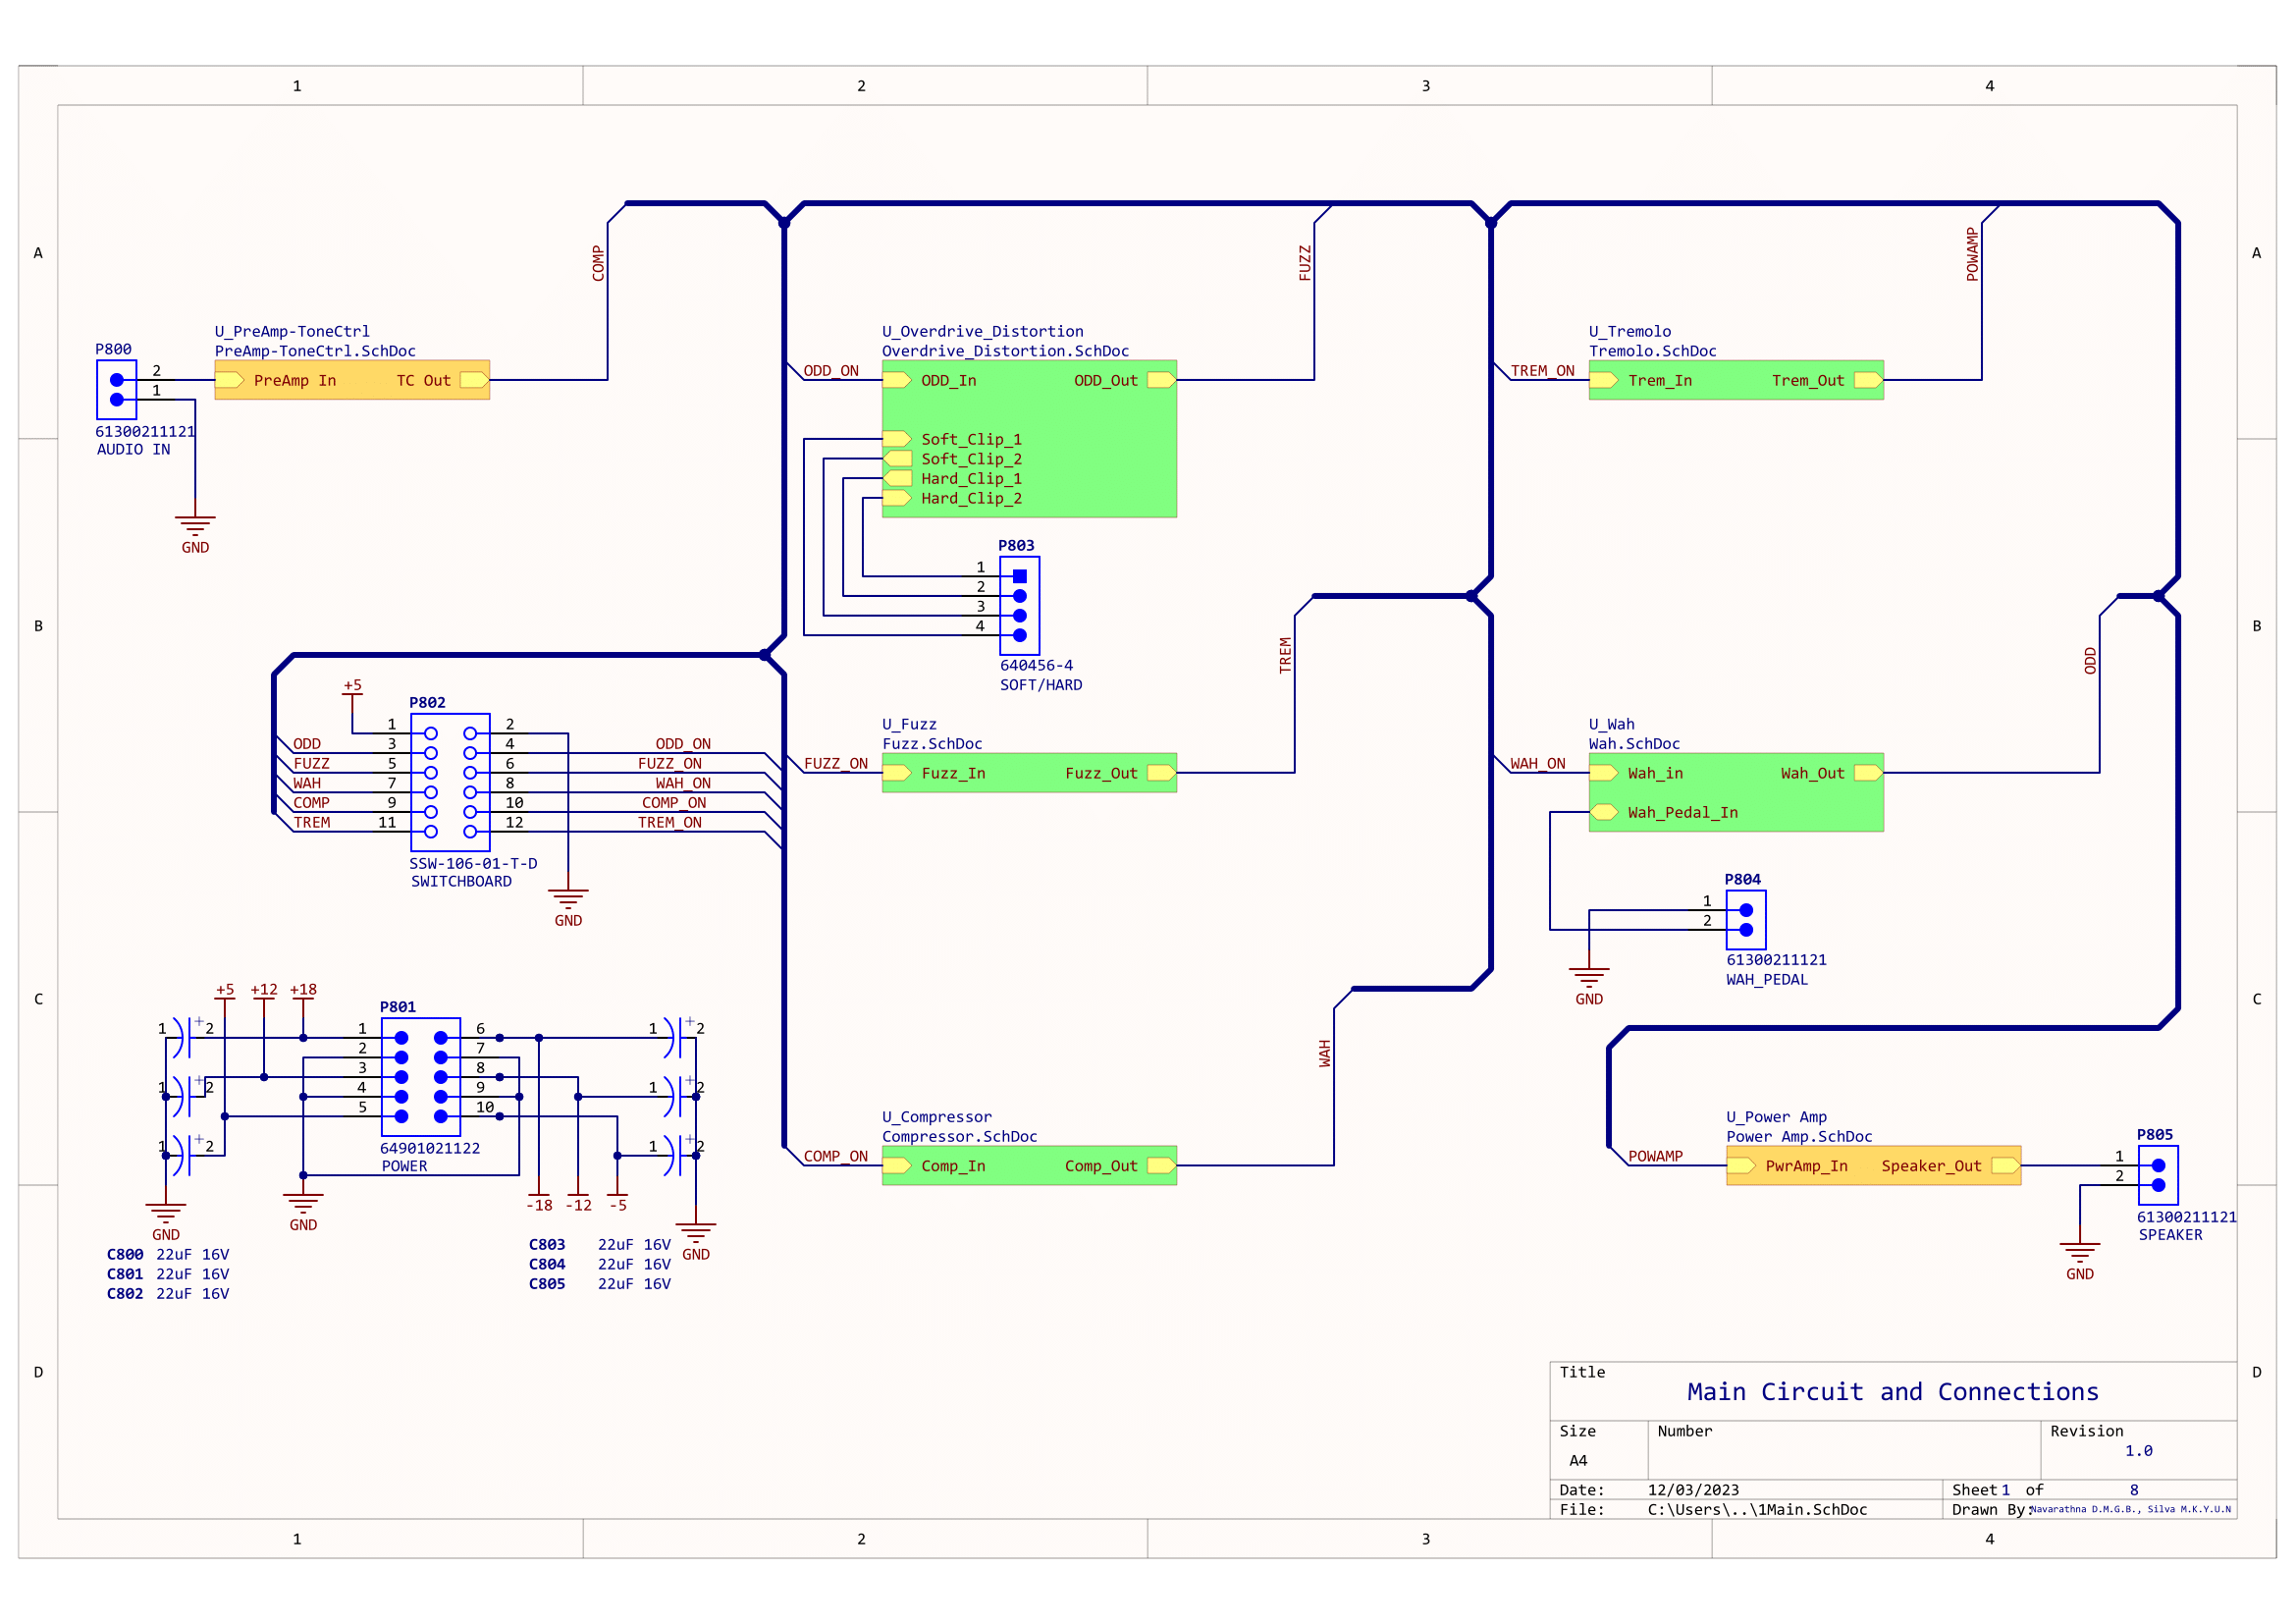
\includegraphics[scale=0.4]{conn.png}
                    \caption{Schematic showing the interconnections between the effects}
                    \label{fig:enter-label}
                \end{figure}
                
                Instead the new setup given above is one of the widely used lineups used by the guitarists. Further we have given the user the ability to switch ON and OFF (bypass) the effect.  
                
                
	\section{Component Selection}
            \textbf{NE5532 Dual Operational Amplifier} is the IC that has been used in the pre amplifier, as this is an operational amplifier which is a low noise amplifier. Since the input to this stage is an extremely weak signal that is usually sent by an instrument over a long wire, more noise gets added. Hence it is important to have lower noise output in this amplification. It also contains a high slew rate. This is specially beneficial to obtain an audio signal of good quality, with higher bandwidth.\\

            \textbf{TL072 Dual Operational Amplifier} is the operational amplifier that has been used in other effects. This IC contains a higher slew rate, and this will be important as the effects add "controlled noise" into the audio, and it would require higher slew rates to facilitate those. Further, TL072 contains short circuit protection, in case which an effect should short circuit accidentally.\\

            \textbf{BC109 NPN Silicon Planar Epitaxial Transistor} is the transistor that has been used in the Fuzz circuit. For the fuzz, the nature of the clipping slightly changes with the transistor, and its characteristic curve. In the original fuzz pedals, old germanium transistors such as NKT275, or AC128 has been used. However as these transistors are not being currently manufactured, and extremely hard to come by, we have used a modern replacement, BC109 that is usually used by manufacturers these days.\\

            \textbf{TDA2040 20W Hi-Fi Audio Power Amplifier} Was used as the operational amplifier in the power amplifier circuit. This was chosen due to its powerful output stage, linearity and low distortion.
            
	\section{PCB Design}
            For the design of this device, we have decided to manufacture it in 3 PCBs:
            \begin{enumerate}
                \item Main PCB (20.5 x 9.5 cm)
                \item Switchboard (18.5 x 3.5 cm)
                \item Power Supply Unit (7 x 7.5 cm)
            \end{enumerate}

            Here the Power Supply was placed further away from the Main PCB, to avoid any possible interference. The Switchboard contains the switches to turn on or off the effects individually. Since this device is usually used by guitarists while playing their instrument operating by their feet. For this, it requires this board to withstand more force compared to others, hence the switches were moved onto a different PCB. \\

            Here the Main PCB is 20.5cm x 9.5cm. Due to the size and possible weight limitations, it was decided to manufacture the PCB locally. Due to the above reason, the PCB design required to have generally larger clearances, and single layered design. However due to the local manufacturing, the PCBs contained a large number of errors that required correcting them by hand.\\

            In designing, the single layering lead to overly elongated tracks which is undesirable due to possible noise addition. This issue was mitigated by using PCB jumpers.\\

            \begin{figure}[h!]
                    \centering
                    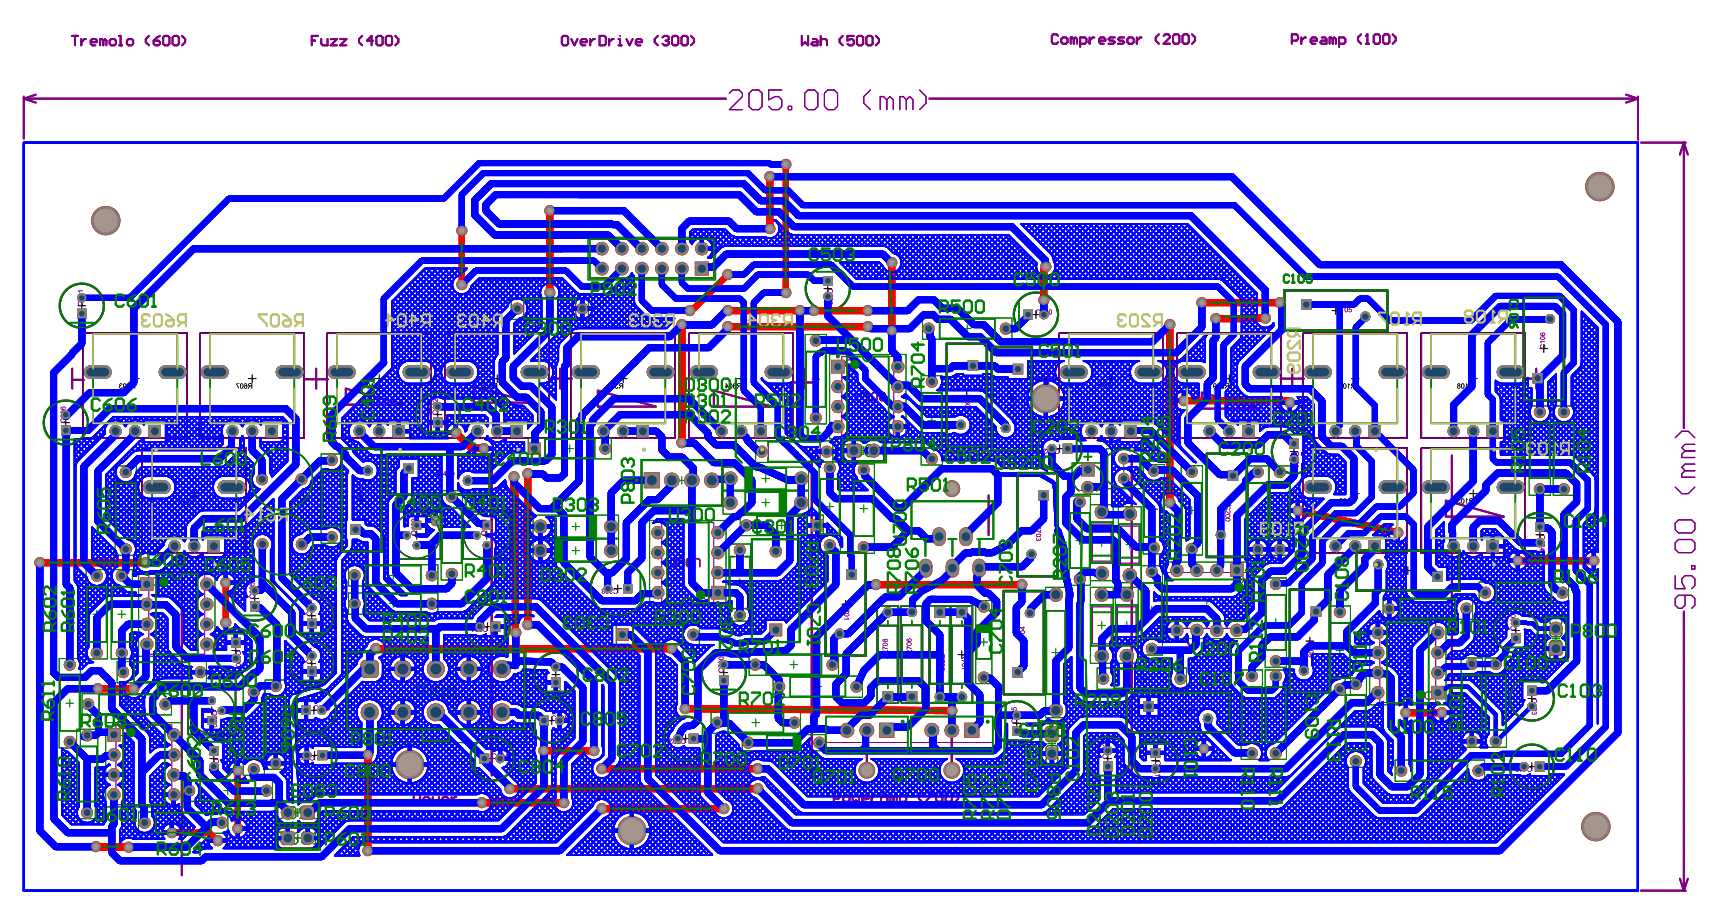
\includegraphics[scale=0.4]{main-1.png}
                    \caption{The layout of the Main PCB}
                    \label{fig:enter-label}
                \end{figure}

            \begin{figure}[h!]
                    \centering
                    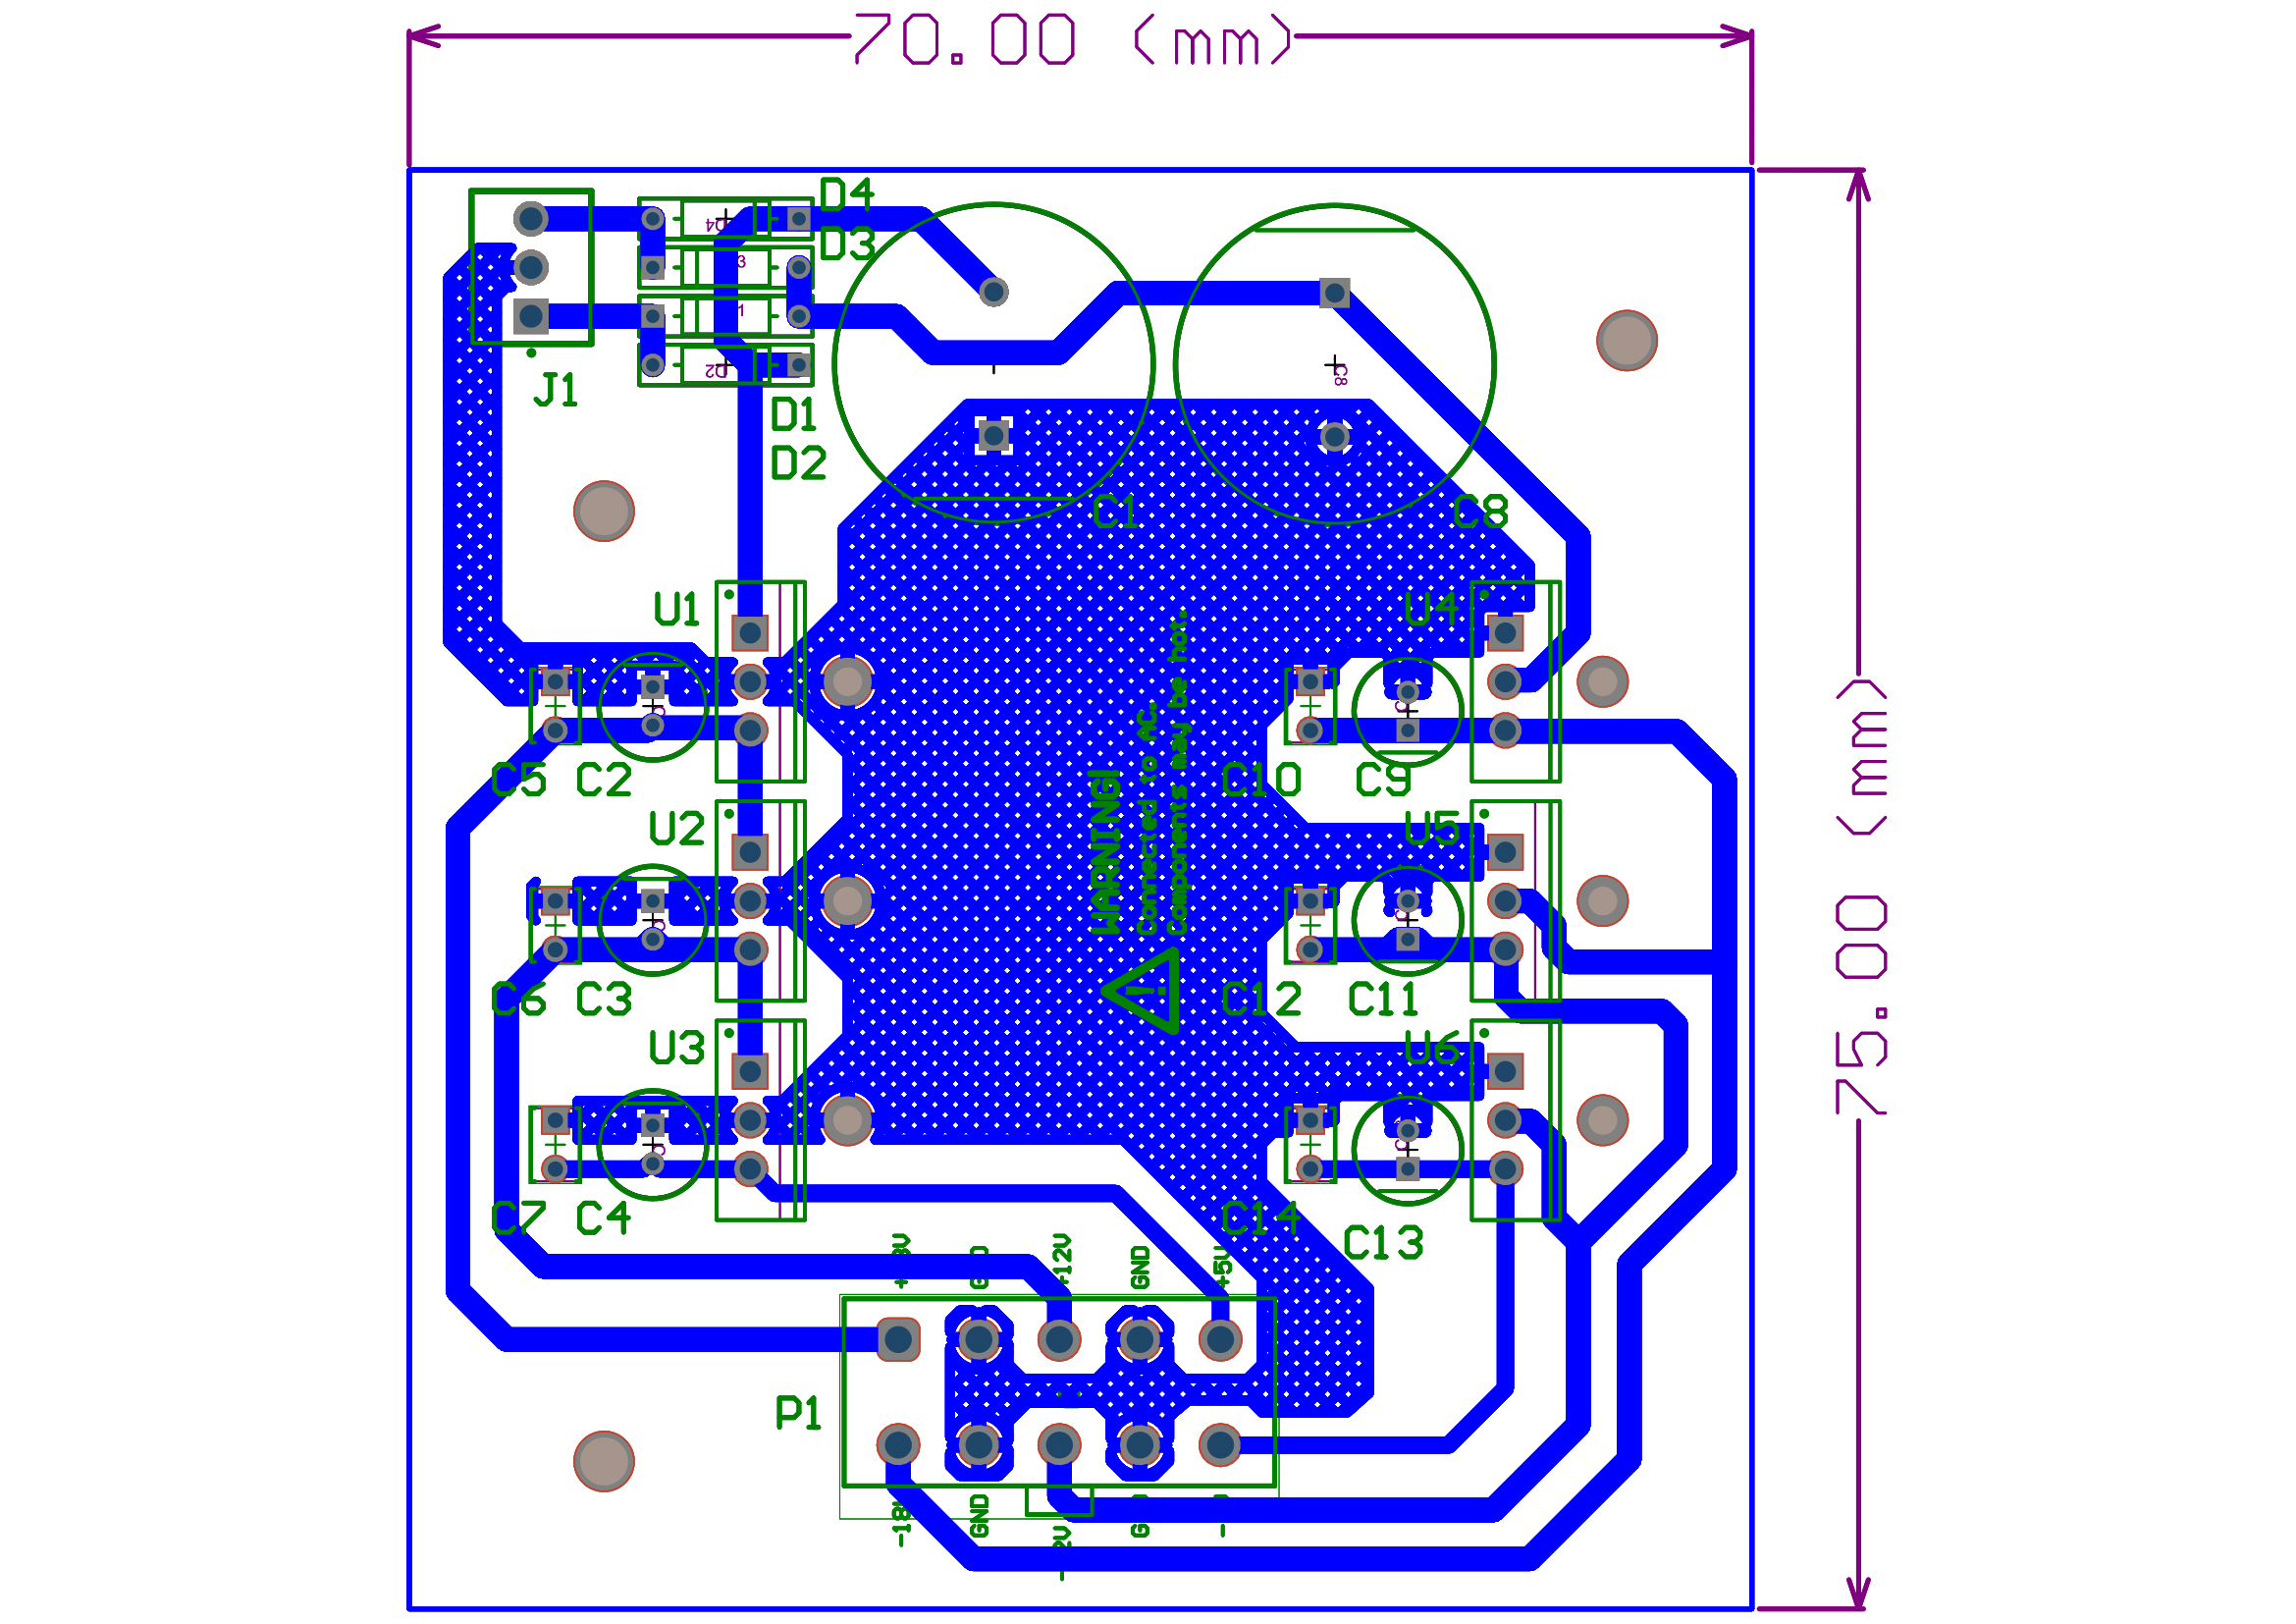
\includegraphics[scale=0.2]{power-1.png}
                    \caption{The layout of the Power Supply PCB}
                    \label{fig:enter-label}
                \end{figure}

            \begin{figure}[h!]
                    \centering
                    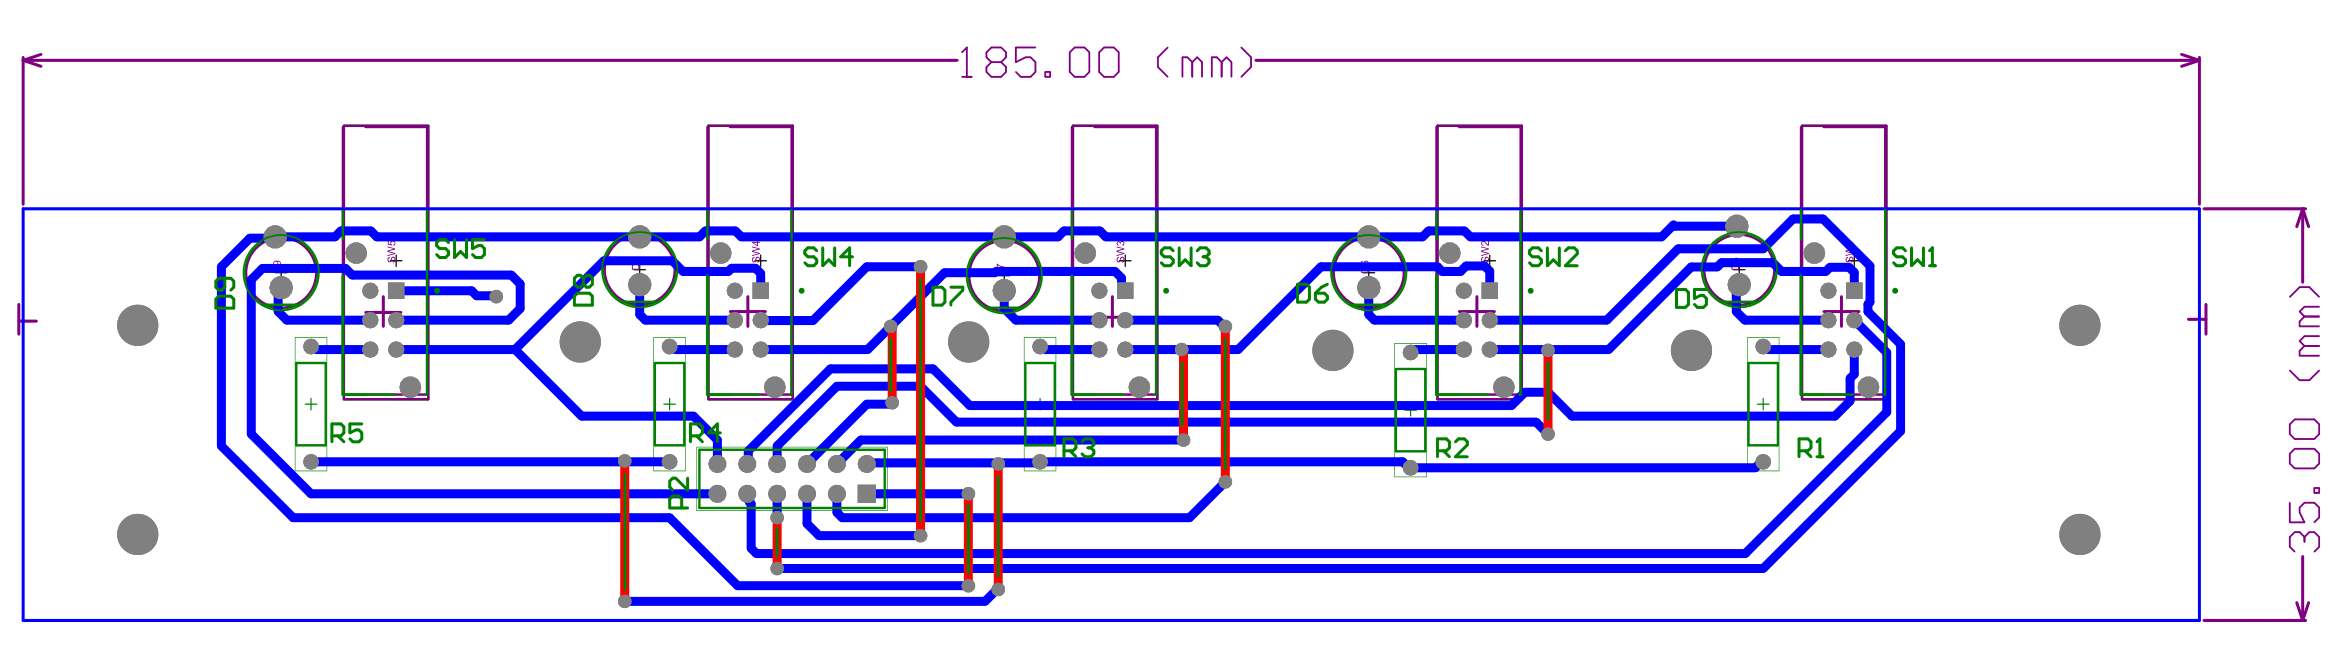
\includegraphics[scale=0.3]{switchboard-1.png}
                    \caption{The layout of the Switchboard PCB}
                    \label{fig:enter-label}
                \end{figure}
            
            As the locally manufactured PCBs had no UV solder mask applied on them, soldering became a challenging task. Having a constant ground plane can cool down the solder joint too fast, making it difficult to solder the joints connected to the ground plane. For this issue, 'relief connect', having only four wires connected to the pad, leaving an air gap. Further the plane is designed to have an hatched pattern, rather than a solid pour which would cool down the joints too fast. 

             \begin{figure}[h!]
                    \centering
                    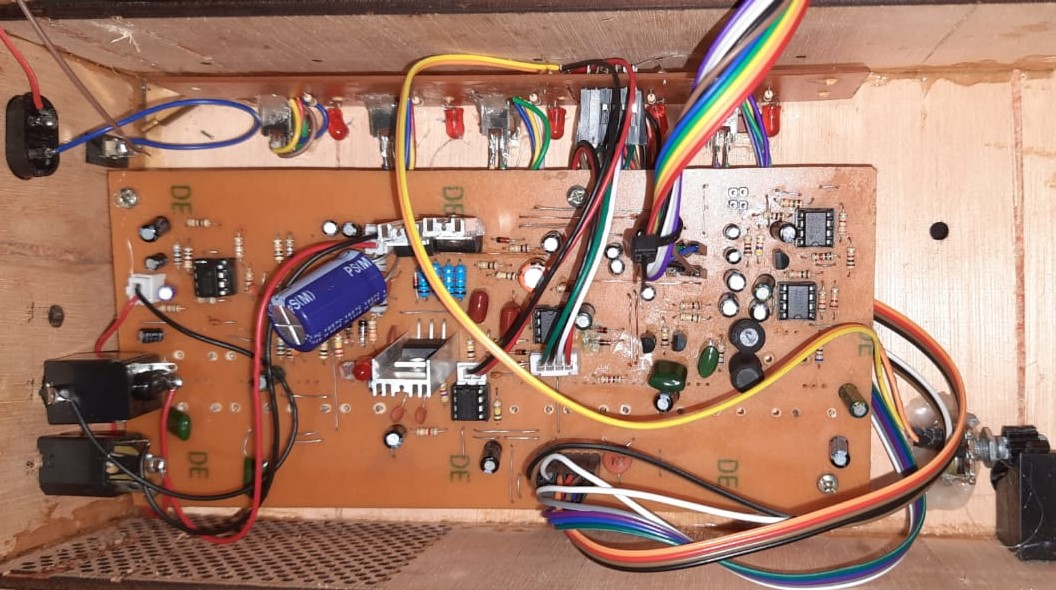
\includegraphics[scale=0.3, origin=c]{4.jpg}
                    \caption{The main PCB and the Switchboard assembled inside the enclosure}
                    \label{fig:enter-label}
                \end{figure}

	\section{Enclosure Design}
            Since most local 3D printers does not support to print up to 30cm continuously it was decided to proceed with a wooden design giving it a more old-fashioned-look. It was able to get the design laser cut onto a wooden board,  in such a way that it could be assembled later.\\

            The Pedal required for the Wah was 3D printed, since it consisted of several intricate parts.

            \begin{figure}[h!]
                    \centering
                    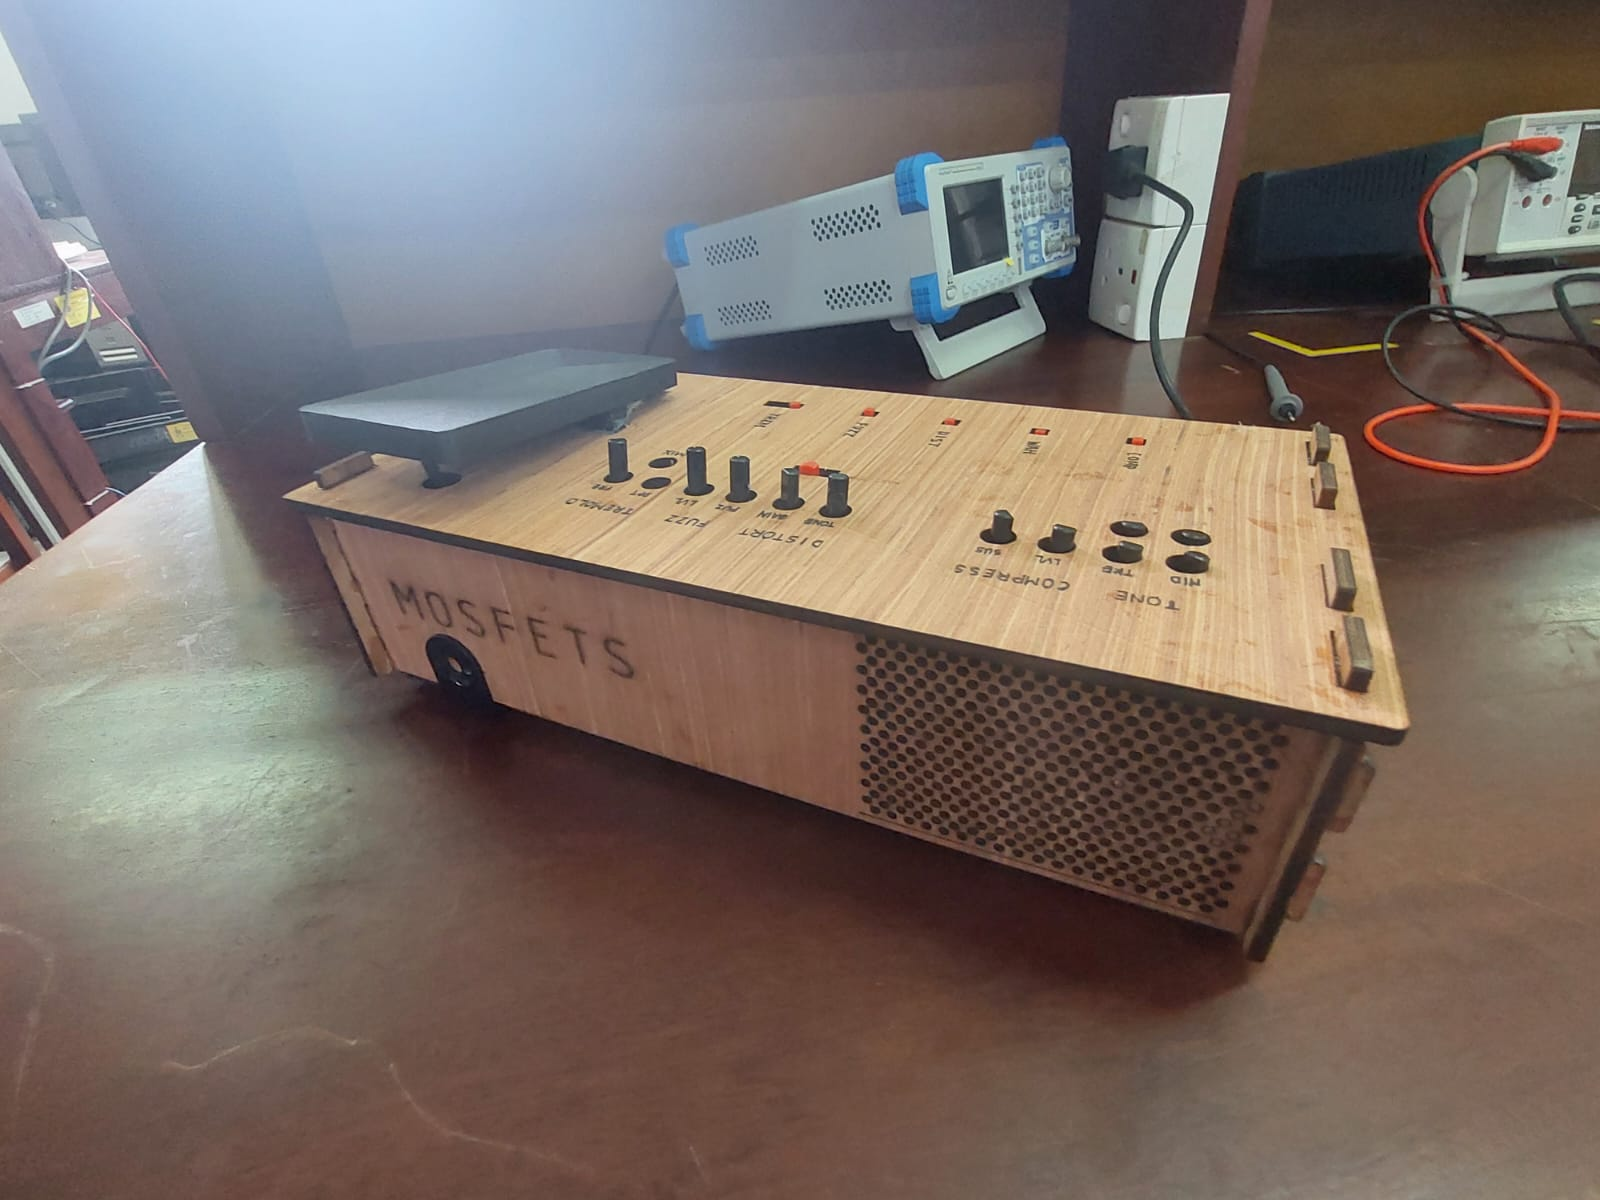
\includegraphics[scale=0.2]{1.jpg}
                    \caption{The wooden enclosure}
                    \label{fig:enter-label}
                \end{figure}

	\section{Software Simulation and Hardware Testing}
            All the circuits except for the compressor were simulated using the simulation software LTSpice before its first hardware implementation.\\\\
            
            During this, stage the changes were done to the circuits to obtain the required conditions. Since this was an audio application, the voltage sources for the input signals were set to sample .wav files of recorded guitar sounds, often consisting of lead parts, chords, single chords and single notes. Then the output of the circuit was set to be saved to another .wav file. Then the circuits were tweaked until the required output is obtained.
            The compressor could not be simulated since the circuit involes an LED and an LDR working in conjuction.\\\\

            Once the simulations were successful, the circuits were implemented on breadboards separately in the laboratories. Even though the breadboards lead to loose connections due to older hardware, the output gave a considerably clean output.

	
	\section{Conclusion \& Future Works}
            Hence it is conclusive that building of a guitar pedalboard by combining several effects is feasible. This gives a cost effective method of adding a several well known 'effects' modifications to the audio signal.\\

            In the future, we expect to modify the circuit using a double layered PCB, which would reduce the size, hence allowing to add more effects. Further we expect to add a method to switch between and reorder the effects, using digital circuitry.
	
	\section{Contribution of Group Members}
            \textbf{Navarathne D.M.G.B.} Fuzz, Power Amplifier and the Switchboard\\\
            \textbf{Senevirathne I.U.B.} Wah, Overdrive/Distortion, and the enclosure design\\\
            \textbf{Silva L.J.J.P.} Pre amplifier, Tone controller, and the Power Supply\\\
            \textbf{Silva M.K.Y.U.N.} Compressor, Tremolo and the PCB design
	
	\section*{Acknowledgment}
            We express our sincere gratitude to Nifla M.N.F., Nima Wickramasinghe and Chirantha Kurukulasuriya for mentoring us through this process. Further we express our gratitude to Eng. Kithsiri Samarasinghe for educating us with his valuable knowledge about operational amplifiers and their workings. 
\end{document}
